%*************************************************************
\chapter{Designtheorie}\label{ch:designTheorie} \index{Design!- theorie}
%*************************************************************

\begin{quote}
	\begin{flushright}{\slshape    
	    >>Schaut man sich die gegenwärtige Lage des Designs an, fällt der eklatante Widerspruch zwischen der Publizität des Desgignbegriffs - nach dem Motto ``Alles ist Design'' - und der Theorielosigkeit des Designs auf.<<} \\ \medskip
	    --- \defcitealias{Bonsiepe:1992}{Gui Bonsiepe}\citetalias{Bonsiepe:1992} \citep{Bonsiepe:1992}
	\end{flushright}
\end{quote}

Anders als in den meisten Professionen, kann die Disziplin \emph{Design} nicht verallgemeinert werden. Es muss stark zwischen der Theorie und der Praxis unterschieden werden. Wer nun eine allgemeine Theorie über Design erwartet, \emph{>>muss zur Kenntnis nehmen, dass eine solche Theorie nicht das intelligible Produkt eines Einzelnen sein kann, sondern allenfalls das Ergebnis einer Designdisziplin sein könnte, welche ihre Praxis reflektiert<<} \citep{Schneider:2008}.

\medskip Im folgenden Kapitel werden daher allgemeine Eigenschaften und Erklärungen von Design erläutert. Im Anschluss wird die Designpraxis, insbesondere von \ac{HCI} und Interaction Design, anhand modellzeigender Designmethoden erfasst.

\section{Was ist Design?} \index{Design}
Fragt man Fachleute verschiedener Abteilungen oder Berufsgruppen nach einer Definition von Design, so wird jeder eine andere Antwort finden. Geradezu jede Art der Kreation – vom Schreiben eines Programms bis zum Erstellen eines Businessplans – kann als Design verstanden werden. Durch diese Vielseitigkeit, ist es schwer eine präzise, nutzvolle Beschreibung zu finden.  Hier beginnt auch die Problematik. \citep{Sagmeister:2008}

\medskip John Heskett schrieb einst: \emph{>>Design is to design a design to produce design<<} \citep{Heskett:2005}. Dies zeigt, wie kompliziert und verwirrend eine Diskussion über Design durch den Begriff an sich bereits sein kann. Design hat so viele Bedeutungen, dass allein das Wort Verwirrung stiftet. Kritisch betrachtet, ist jedoch der Gebrauch des Wortes an jeder Stelle des Zitates grammatikalisch richtig. Das erste ist ein Nomen und beschreibt Design als generellen Überbegriff, wie z.B. in: >>Design ist wichtig für die Wirtschaft.<< Das zweite ist ein Verb und steht für eine Tätigkeit bzw. Prozess, wie z.B. in: >>Sie hat den Auftrag einen neuen Mixer zu designen.<< Das dritte ist wiederum ein Nomen, welches diesmal für ein Konzept bzw. einen Vorschlag steht, wie in: >>Das Design wurde dem Auftraggeber zur Freigabe vorgelegt.<< und das letzte ist wieder ein Nomen, das für ein fertiges Produkt steht, welches durch das Konzept umgesetzt wurde. Wie z.B.: >>Der neue VW Beetle lässt klassisches Design neu aufleben.<< \citep{Heskett:2005}\\
Durch diese Zerlegung kann man erkennen, dass sich der Begriff Design in zwei große Teilbereiche unterteilen lässt. Zum einen in die ursprüngliche Philosophie von Design - als Tätigkeit bzw. Prozess um ein Produkt zu entwickeln - und zum anderen in die Repräsentation eines Produkts. Webster beschreibt diesen Zusammenhang beider Bereiche wie folgt:
\begin{quote}
\slshape >>A design is an information base that describes aspects of this object, and the design process can be viewed as successive elaborations of representations, such as adding more information or even backtracking and exploring alternatives.<< 
\begin{flushright}\citep{Webster:1988}\end{flushright}
\end{quote}

\subsection{Design als Prozess} \index{Design!als Prozess}
Nach Webster ist der Designprozess eine schrittweise Ausarbeitung von Repräsentationen. Wann findet aber nun diese >>Ausarbeitung<< innerhalb eines Projektzyklus statt und was soll sie beinhalten?\\
Im Projektmanagement, welches sich mit der Gesamtheit an Aufgaben, Techniken, Mitteln etc. für die Abwicklung eines Projekts beschäftigt, spricht man dabei auch von der Designphase\index{Design!- phase}. Es gibt zwar Ansichten, dass die Designphase gleich der Entwicklungsphase ist, jedoch sind meist das die Projekte, die am Ende scheitern oder Schwierigkeiten haben, das Projekt in angegebener Zeit mit vordefiniertem Budget zu beenden.

\medskip Um ein Produkt zu entwickeln sollte man sich ausführliche Gedanken über die aufkommenden Probleme und um die Umsetzung zur Bewältigung dieser machen. Viele Projektmodelle wie z.B. das Wasserfallmodell\index{Wasserfallmodell} berücksichtigen bereits diesen Schritt. Jedoch gehen all diese Modelle von standardisierten Entwicklungsschritten aus, die zeitlich sequentiell durchlaufen werden sollen. Die Ergebnisse der Analyse- bzw. Forschungsphasen werden dabei in Dokumenten festgelegt um die weitere Entwicklung zu leiten und zu unterstützen. Das Zurückgreifen auf vergangene Phasen ist hier nicht erlaubt, jedoch in der Praxis die Regel und resultiert auf sog. >>Entwicklungsfehler<<.
Genau hier sollte das Umdenken beginnen. Die zwei (leider) gebräuchlichsten Mythen in der Industrie sind: 
\begin{quote}
	\begin{enumerate}
		\item \textsl{>>That we know what we want at the start of a project<<}, und
		\item \textsl{>>That we know enough to start building it<<.}
	\end{enumerate}
	\begin{flushright}\citep{Buxton:2007}\end{flushright}
\end{quote}

Die Realität sieht aber anders aus. Vor der Entwicklung werden einem nicht alle Probleme offenbart, welche im Projektverlauf auftreten, sondern lediglich Grundprobleme. Es ist im Vorhinein nicht möglich eine ganzheitliche Analyse durchführen ohne nicht auch Entscheidungen zu treffen, welche Analysen beeinflussen. Aus diesem Grund sollte der Designprozess durchgehend im Projektablauf verankert sein.
\autoref{fig:buxtonProductDevProcess} zeigt ein mögliches Modell eines Produktentwicklungsprozesses. Der	Designprozess	(in	rot gehalten) erstreckt sich hierbei über alle Phasen im Projekt bis zum Verkauf und beinhaltet das Design der Business- und Entwicklungspläne, sowie das Design des Produkts an sich. Plump	gesprochen ist die Hauptaufgabe	des	Designprozesses das Auffinden und Lösen von Problemen. Je nach Aufgabenstellung und Art des Projektes variieren naturgemäß die Probleme und somit auch die Aufgaben von Design als Tätigkeit. 

\begin{figure}
        {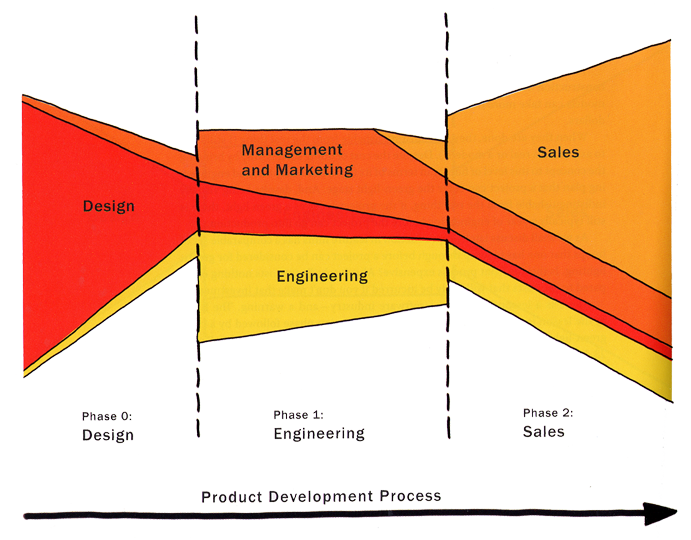
\includegraphics[width=\linewidth]{gfx/buxtonProductDevProcess}}
		\caption[Der Produktentwicklungsprozess \newline \citep{Buxton:2007}]{Der Produktentwicklungsprozess unterteilt in seine Verantwortungsbereiche. Von zentraler Bedeutung ist der Begriff Design, der das Design der Business- und Entwicklungspläne, sowie des Produkts selbst einschließt.}\label{fig:buxtonProductDevProcess}
\end{figure}

\subsection{Design als Repräsentation} \index{Design!als Repräsentation}
Das Entwickeln verwendbarer Repräsentationen eines Produkts ist essenziell im Designalltag. Repräsentationen können formal oder formlos, exakt oder vage sein und dienen verschiedenen Zwecken innerhalb des Designablaufs. Designer sollten zum einen die Fähigkeit besitzen eine passende Darstellung bzw. Repräsentation für ihre Aufgaben zu wählen, und zum anderen in der Lage sein diese auch richtig einzusetzen.
Im Laufe eines Produktdesigns können verschiedene Repräsentationen bzw. Modelle innerhalb des Designprozesses von Nöten sein. Ein gutes Modell ist präzise genug um die Eigenschaften des Systems wiederzuspiegeln, und einfach genug um Verwirrung zu vermeiden. Es verwendet eine Art der Repräsentation welche zum Zweck passt.
Die Wahl passender Modelle und das Konstruieren dieser, ist ein schwieriger aber wichtiger Teil der Arbeit von Designern. Sie müssen dabei stets beachten, wie das Modell verwendet werden soll und wer es benutzen wird. Deswegen sollte auch die Modellierungstechnik auf den Abstraktionsgrad und den >>Empfänger<< (der mit dem Modell arbeiten wird) angepasst werden. \citep{Preece:1994}
Wie im allgemeinen Produktdesign gibt es auch speziell im Softwaredesign eine große Menge an Repräsentationsarten bzw. Techniken, welche die Aufmerksamkeit auf verschiedene Aspekte des Designs lenken können. Auf diese Techniken, auch Designmethoden genannt, auf welches später eingegangen wird.

\subsection{Designdisziplinen} \index{Design!- disziplinen}
Design umfasst eine große Anzahl an verschiedenen Disziplinen. Sei es Produkt- bzw. Industriedesign, Kommunikationsdesign, Softwaredesign oder Modedesign, sie alle beinhalten auf ihrem Gebiet fachmännische Fähigkeiten und dienen zur Unterscheidung von Kompetenzen professioneller Designer. Über die Jahre kristallisierten sich ebenfalls die unterschiedlichsten Arbeitsfelder\index{Design!Arbeitsfelder} heraus. Das für Softwaredesign bedeutungsvollste der letzten Jahre ist (User) Interface Design bzw. Interaction Design, auf welche sich der folgende Text bezieht.\\
Um Interface Design beschreiben zu können, ist es vorerst nötig den Begriff des User Interfaces zu definieren. Das User Interface eines Systems besteht aus dem System selbst, dem Benutzer des Systems und der Weise, in der sie aufeinander einwirken. Es enthält somit Elemente die Teil des Systems sind, Elemente die ein Teil des Benutzers sind und Kommunikationsmethoden um Informationen von einem Ort zum anderen zu bringen.

\medskip Wie \autoref{fig:sagmeisterUI} zeigt, gibt es eine Grenze zwischen den Elementen des Systems, die Teile des User Interfaces sind und	denen, die für	die	internen Funktionen des Systems stehen. Das finden der passenden Grenze ist Aufgabe des	Designers und fällt	in den Aufgabenbereich	von	User Interface Design \citep{Barfield:1993}. Es befasst sich also mit der Entwicklung passender Benutzerschnittstellen zwischen Mensch und Maschine.

\begin{figure}
	\begin{center}
        {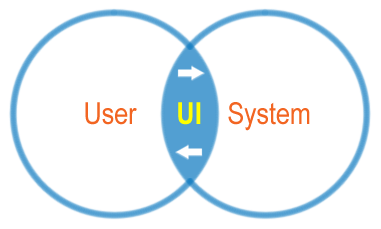
\includegraphics[width=.7\linewidth]{gfx/sagmeisterUI}}
	\end{center}
		\caption[Visualisierung des User Interfaces \newline \citep{Sagmeister:2008}]{Visualisierung des User Interfaces. Das User Interface, welches aus dem System und dem Benutzer geformt wird, stellt Methoden zu Verfügung um die Kommunikation beider Seiten bestmöglich zu unterstützen. Das Finden einer passenden Grenze von Funktionen, die zum Interface oder intern zum System gehören, ist Aufgabe von User Interface..}\label{fig:sagmeisterUI}
\end{figure}

\medskip Interaction Design beschäftigt sich ähnlich wie Interface Design mit dem Verhalten von Mensch und Maschine. Jedoch spezialisiert es sich auf die Wechselwirkungen bzw. Interaktionen zwischen Menschen, welche durch Verbindungen mit maschinellen Produkten entstehen. Der Zusammenhang zwischen User Interface Design/Engineering bzw. Interaction Design ist in \autoref{fig:safferInteractionDisciplines} ersichtlich. Sie zeigt ebenfalls verwandte Disziplinen, wie \emph{Information architecture}, \emph{Communication design}, \emph{Usability engineering} oder \emph{Human-computer interaction}, welche sie nicht nur beeinflussen, sondern auch Teil von ihnen sind. Man merkt somit wie schwierig es ist, Disziplinen, die zwar separat existieren aber sich mit vielen anderen Disziplinen überschneiden, abzugrenzen und ihre Funktionen zu beschreiben. Nicht jede Organisation benötigt einen Spezialisten für jede Disziplin. Eine Person, möge er sich Informationsarchitekt oder Interface Designer nennen, kann und wird höchstwahrscheinlich in mehreren Disziplinen, je nach Bedarf tätig sein. \citep{Saffer:2007}

\begin{figure}
	\begin{center}
        {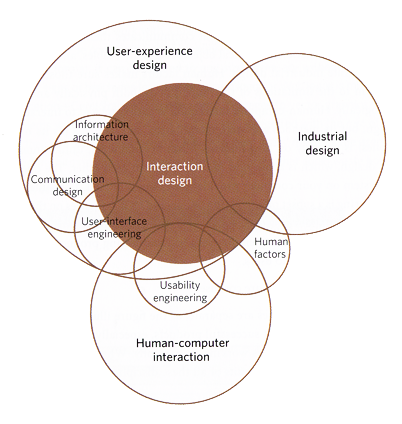
\includegraphics[width=.8\linewidth]{gfx/safferInteractionDisciplines}}
	\end{center}
		\caption[Verwandte Disziplinen von Interface- und Interaction Design \newline \citep{Saffer:2007}]{Verwandte Disziplinen von Interface- und Interaction Design. Sie beeinflussen nicht nur, sondern sind auch Teil von Interface bzw. Interaction Design. Die Schwierigkeit	Disziplinen abzugrenzen, zeigt den interdisziplinären Charakter, den Designer an den Tag legen.}\label{fig:safferInteractionDisciplines}
\end{figure}

\medskip Zu diesen zählen ebenfalls andere akademische Disziplinen, wie z.B. im sozialen, technologischen oder organisatorischen Sektor, wie \autoref{fig:benyonDisciplines} veranschaulichen soll.\\
Natürlich ist es nicht nötig, dass Designer alle Fähigkeiten zur Erstellung von Designs besitzen - vor allem da das Designen von Interaktiven Systemen meist Aufgabe eines ganzen Teams ist - jedoch müssen sie in der Lage sein, Techniken anderer Disziplinen	anwenden	zu können bzw. wenn nötig die Mittel zur Erforschung dieser besitzen. \citep{Benyon:2005}

\begin{figure}
        {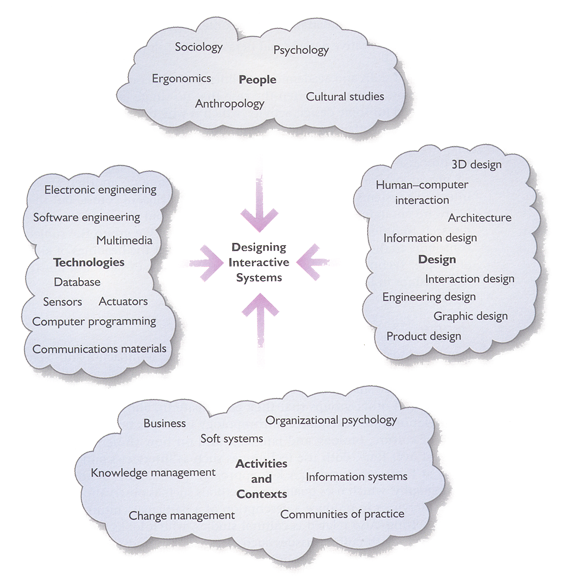
\includegraphics[width=\linewidth]{gfx/benyonDisciplines}}
		\caption[Miteinfließende Disziplinen im Interaktiven System Design \newline \citep{Benyon:2005}]{Miteinfließende Disziplinen im Interaktiven System Design. Sie verkörpern Bereiche aus welchen Designer Techniken beziehen	und anwenden. Es ist zwar nicht nötig, dass Designer jeweils alle Fähigkeiten besitzen müssen, jedoch sollten sie wenn nötig die Mittel zur Erforschung dieser besitzen.}\label{fig:benyonDisciplines}
\end{figure}

\medskip Im Allgemeinen lässt sich aber User Interface- bzw. Interaction Design wie folgt beschreiben:

\begin{quote}
	\textsl{>>The design of the subjective and qualitative aspects of everything that is both digital and interactive.<<}
	
	\smallskip oder allgemeiner: 
	\smallskip
	
	\textsl{>>The design of everything that is both digital and interactive.<<}
\begin{flushright}\citep{Moggridge:2007}\end{flushright}
\end{quote}

\subsection{Der kollaborative Charakter} \index{Design!- kollaboration}
Designkollaboration wird durch die soziale Welt geformt. Aus diesem Grund ist es unmöglich Designspezifikationen und Artefaktbeschreibungen zu interpretieren, ohne die soziale Situation in der sie erstellt wurden zu verstehen \citep{Brown:2002}. Da Design immer mit Kommunikation und Interaktion - zwischen Einzelpersonen und Gruppen in komplexen sozialen Situationen - zusammenhängt, können die technischen Ergebnisse nicht vom sozialen Charakter der Designaktivitäten getrennt werden. Er ist durchgehend in Meetings, Diskussionen, Argumenten, Debatten und Interpretationen vorhanden und macht das dichtverflochtene Gewebe von Design aus. Minneman beschreibt in diesem Zusammenhang Design als \emph{>>social contruction of a technical reality<<} \citep{Minneman:1991}.

\medskip Kollaborative Wissenskonstruktion ist wichtig für ein erfolgreiches Design. Zudem ist es auch wichtig, Mehrdeutigkeiten zu bewahren, um Teammitglieder Freiheiten zu ermöglichen.

\begin{quote}
	\textsl{>>[It is important to provide team members with] the freedom to manoeuvre independently within objects worlds and providing room for the recasting of meaning in the negotiations with others.<<}
\begin{flushright}\citep{Bucciarelli:1994}\end{flushright}
\end{quote}

\medskip Eine erfolgreiche Kollaboration zeichnet sich durch die Bildung eines gemeinsamen Verständnisses aus. Clark und Brennan benutzen den Begriff \emph{Grounding} um diesen Vorgang zu beschreiben, in dem das Kommunizierte auch verstanden wird. Sie erklären weiters: \emph{>>all collective actions are built on common ground and its accumulation<<}, womit sie betonen, dass Gemeinsamkeiten kontinuierlich von Moment zu Moment durch die Interaktion der Teammitglieder aufgebaut werden \citep{Clark:1991}. Diese Interaktionen treten in verschiedenen Formen auf und beeinflussen den kollaborativen Designprozess. Short et al. nennen in \citep{Short:1991} beispielsweise Aspekte der visuellen Kommunikation, welche soziale Interaktionen beeinflussen: 

\begin{quote}
	\textsl{>>In normal face-to-face interaction, the participants exchange in addition to the verbal material, a range of non-verbal cues such as facial expression, direction of gaze, posture, dress and physical distance.<<}
\begin{flushright}\citep{Short:1991}\end{flushright}
\end{quote}

Um also ein Verständnis über Designkollaboration zu bekommen, müssen Gemeinsamkeiten, in Hinsicht auf Relevanz und Bedeutung der in kollaborativen Designaktivitäten vorgebrachten Informationen, erlangt werden \citep{Hill:2001}.

\subsection{Designvokabular} \index{Design!- vokabular}
In einer Studie über Industrial Designer, die an Konzeptskizzen arbeiteten, fanden Pan et al. \citep{Pan:2002} heraus, dass die Designer die Formen ihres Designs auf verschiedene Weisen verbal beschrieben. Ihre Sprache war nicht klar, einheitlich oder im Allgemeinen verständlich für Außenstehende. Designer haben ein \emph{>>creative vocabulary, which has rich meanings in design communication<<}\citep{Pan:2002}. In Hinsicht auf globale Kollaborationen zwischen einzelnen Arbeitsgruppen, ist der Wunsch an ein gemeinsames Designvokabular naheliegend. Laut Hill \citep{Hill:2001} baut der Erfolg von Designteams stark auf die folgende Fähigkeit der Teilnehmer auf: \emph{>>negotiate different design perspectives and specialities<<}. \emph{>>Similarities in voice<<} ist das Um und Auf, bei Teammitglieder mit verschiedenen Disziplinen und Hintergründen.

\medskip Das Definieren eines gemeinsamen Designvokabulars scheint aber doch eher utopisch. Bucciarelli meinte dazu, dass auch wenn Teilnehmer die gleiche gemeinsame Sprache (wie z.B. Englisch) verwenden, kann die Sprache auf verschiedene Weisen angewendet werden, wodurch es scheint als würde ein Teilnehmer einer andere Sprache sprechen:

\begin{quote}
	\textsl{>>Not different in the sense that for you, as a foreigner, a translation would make meanings clear \ldots but different in that the concepts and ideas and relationships among the things of an opbject world require new leaning, like the learning of a foreign language.<<}
\begin{flushright}\citep{Bucciarelli:2002}\end{flushright}
\end{quote}

Im Grunde bedeutet dies für Designteams (speziell für globale), dass sie nicht nur eine sprachliche Hürde von z.B. Personen unterschiedlicher Herkunft meistern müssen, sondern auch von Personen, die von komplett unterschiedlichen Objektwelten stammen - abhängig von kulturellen Hintergrund, der Ausbildung und professionellen Disziplinen.

\medskip Larsson hält \emph{Negotiation} als adequateren Begriff, um die Kommunikation zwischen den einzelnen Mitgliedern eines Designteams zu beschreiben, da die Teilnehmer aktiv den Kontext und Inhalt der Situationen formen und die Informationen nicht passiv mit eindeutigen Bedeutungen und definierten Settings übertragen. \citep{Larsson:2003} \\
Die Wissenskonstruktion ist ein kollaborativer Prozess, der wie bereits Bucciarelli beobachtete, aus einer inhärenten Mehrdeutigkeit besteht, welche Designer vor die folgende, alles andere als einfache Aufgabe stellt: 

\begin{quote}
	\textsl{>>frequently bringing the results of their object world efforts, which no doubt will conflict, into coherence if design is to proceed - and they must do this without a shared proper language.<<}
\begin{flushright}\citep{Bucciarelli:2002}\end{flushright}
\end{quote}

\subsubsection{Storytelling} \index{Storrytelling}
Eine Art um Verständnis unter Designern zu vermitteln, ist das Erzählen von Geschichten. Geschichten ermöglichen Designer gezielter zu erklären, was sie gerade machen, im Gegensatz zu dem was sie machen sollten - falls sie sich an normative Designmodelle halten. Auch wenn die Geschichten nicht direkt ein Problem lösen, helfen sie dennoch ein gemeinsames Vokabular aufzubauen, um über das Design sprechen zu können. Sie kreieren \emph{>>a new language capable of describing aspacts of the evolving design<<} \citep{Lloyd:2000}.

\medskip Vereinbarte Geschichten ermöglichen Designer verschiedener Sparten, ein gemeinsames Verständnis zu kreieren, auf das sie sich beziehen können, ohne dabei zu konkreten Thematiken zustimmen zu müssen. Es sind konkrete Beispiele, auf die sich Personen mit verschiedenen Hintergründen beziehen können. Da uns das formlose Naturell von Geschichten dazu bringt sie nicht zu ernst zu nehmen, dienen sie als eine gemeinsam verfügbare Wissensquelle - die Freiraum für Interpretation und Fragestellungen aller Beteiligten zulässt \citep{Erickson:1996}. Wie in Orrs Studie über Service Techniker \citep{Orr:1986} beobachtet wurde, dienen Geschichten auch dem Zweck, Erfahrungen zu erhalten und zu verbreiten. Somit bieten sie Grundgerüst für Problemlösungsaktivitäten.

\medskip Zusätzlich bilden sie ein Transportmittel für Gedanken, da sie durch ihre Nutzung, nicht nur anderen etwas beschreiben, sondern auch uns selbst \citep{Norman:1994}.

\subsubsection{Indexical Expressions} \index{Indexical Expressions}
Neben Geschichten, die nützlich bei der Verständnisvermittlung sind, benutzen Designer auch \emph{Repräsentationen}, wie Markierungen oder Symbole, die etwas bestimmtes darstellen und ihnen bei ihren Argumentationen helfen \citep{Norman:1994}. Repräsentationen bieten auf die gleiche Weise wie Geschichten konkrete Beispiele, welche die Gedanken der Designer abbilden. Dabei benutzen sie vorhandene Tools, die die Verständnisvermittlung zwischen den Teammitgliedern im jeweiligen Moment am besten unterstützen.

\medskip In Hinsicht auf ein gemeinsames Designvokabular muss man zur Kenntnis nehmen, dass einige Teile des Vokabulars keine strikten Definitionen haben. Designer und auch andere Personen, benutzen \emph{Indexical Expressions} wenn sie kommunizieren. Eines muss man sich dabei aber vor Augen halten:

\begin{quote}
	\textsl{>>[Indexical Expressions] cannot straightforwardly be repeated or reused outside the context in which they originated, without changing their meaning.<<}
\begin{flushright}\citep{Kristoffersen:1999}\end{flushright}
\end{quote}

Beispielsweise \graffito{Markierungen und Symbole verlieren außerhalb des Kontextes ihre Bedeutung.} können Wörter wie >>hier/dort<<, >>dies/das<<, >>sein/seine<< oder >>jetzt/dann<< nicht angemessen gedeutet werden, ohne zu wissen unter welchen Umständen sie benutzt wurden \citep{Larsson:2003}.

\medskip Designvokabular dient aber nicht nur zur Verständigung, sondern ist vielmehr ein Hilfsmittel, das Designer bei ihren Arbeitsmethoden begleitet und mit diesen zusammenspielt. \emph{Storytelling} und \emph{Indexical Expressions} deuteten bereits auf essentielle Designmethoden hin, welche im folgenden Abschnitt genauer betrachtet werden.

\section{Designmethoden} \label{sec:designmethoden} \index{Design!- methoden}
Vorstellungskraft ist grundlegend für effektive Designarbeiten. Sie hilft, Dinge aus einem anderen Blickwinkel zu sehen und Designkonzepte bzw. Ideen mit anderen zu erforschen. Verschiedenste Repräsentationen von Designideen können in verschiedenen Etappen für verschiedene Menschen nützlich sein und ihre Vorstellungen beeinflussen. Sie helfen beim Finden, Austauschen und Auswerten von Ideen.

\medskip Es gibt viele Techniken bzw. Methoden, die benutzt werden können um Designprobleme zu verstehen und mögliche Lösungen zu entwickeln. Keine dieser Methoden führt höchstwahrscheinlich zum perfekten Design, aber zu einer Art Dokument oder Darstellung, die benutzt werden kann um sich besser mit Auftraggebern, Benutzern und Kollegen zu verständigen. Verständigung ist es auch, wodurch Lösungen entstehen, ausgewertet, und eventuell zum Endprodukt umgewandelt werden \citep{Benyon:2005}.

\medskip Es werden im folgenden nun wichtige Methoden und Hilfsmittel für Designer beschrieben und Einblicke über deren Grundfunktionsweise geboten. Welche Techniken aber in einem Projekt tatsächlich Anwendung finden, hängt von mehreren Faktoren ab: die Herangehensweise an die Arbeit des Entwicklungsteams, die Art des Projekts, die zur Verfügung stehenden Hilfsmittel etc. Das Auswählen von passenden Methoden bzw. Repräsentationen ist Aufgabe des Designers und erfordert Geschick, um sie auch gut einsetzen zu können. Dabei sollte aber nicht die Repräsentation an sich, sondern die Vorstellungskraft und das Verständnis im Vordergrund stehen, geistig und vor allem erfahrungsmäßig. \citep{Sagmeister:2008} 

\begin{quote}
	\textsl{>>Experience is a very dynamic, complex and subjective phenomenon. It depends upon the perception of multiple sensory qualities of a design, interpreted through filters relating to contextual factors. For example, what is the experience of a run down a mountain on a snowboard? It depends upon the weight and material qualities of the board, the bindings and your boots, the snow conditions, the weather, the terrain, the temperature of air in your hair, your skill level, your current state of mind, the mood and expression of your companions. The experience of even simple artefacts does not exist in a vacuum but, rather, in dynamic relationship with other people, places and objects.<<}
\begin{flushright}\citep{Buxton:2007}\end{flushright}
\end{quote}

\subsection{Artefakte} \index{Artefakte}
Harrison und Minneman beobachteten in \citep{Harrison:1996}, dass Objekte wesentliche Bestandteile von Designkommunikation sind, da sie einen Teil des \emph{Repräsentationspools} von Designer ausmachen. Diese Objekte oder auch Artefakte genannt, können praktisch alles sein; z.B. ein Stift, ein Sessel, eine Zeichnung, oder ein einfaches Blatt Papier. Im Konzeptdesign sind diese besonders wichtig, da in diesem Stadium des Produktentwicklungsprozess noch kein >>gemeinsames<< Designobjekt existiert \citep{Tuikka:2001}. Aus diesem Grund muss ein gemeinsames Artefakt erst durch Kollaboration konstruiert werden, um Diskussionen über Designoptionen und Ideen zu ermöglichen. \citep{Larsson:2003}

\medskip Artefakte sind ein bewehrtes Mittel in \ac{HCI} und \ac{CSCW}. Verschiedene Studien zeigen, das sie eine große Rolle in kooperativen Arbeiten spielen (vgl. \citealp{Bardram:2005, Heath:1992, Hutchins:1995, Robinson:1993, Schmidt:2002, Sellen:2003, Shapiro:1994, Vyas:2008}). Die Forschung und Literatur (z.B. \citealp{Randall:2007}) beschäftigt sich dabei vorwiegend mit drei Hauptaspekten im Bezug auf Artefakte bei der Arbeit: dem \emph{ökologischen}, dem \emph{koordinativen} und dem \emph{organisatorischen}.

\medskip \emph{Ökologisch.} Die Umwelt von Artefakten kann einiges über die Arbeitspraktiken von Personen aussagen. Der Ort, die Position, der Aufbau und die Ausrichtung der Artefakte erlaubt uns zu verstehen was und wie gearbeitet wird. Verschiedene \ac{CSCW} Studien \citep{Heath:1992, Sellen:2003} zeigten, dass die Organisation des Arbeitsbereiches Auswirkungen auf die Arbeit haben. Kidd \citep{Kidd:1994} zeigte, dass die ökologische Struktur von Artefakten eine >>primitive Sprache<< bildet, welche Arbeit erklärt. Er vertritt den Standpunkt, dass die persönliche Anordnung von Artefakten (wie z.B. Papier), Personen befähigt ein besseres Verständnis aufzubauen, da sie so ein Gesamtbild ihrer Arbeit bekommen. Ebenso werden Aufbewahrungsmöglichkeiten, wie z.B. Papierstapel oder -mappen, zu externen Repräsentation, die zusätzliches Verständnis vermitteln und bewahren. Der physische Kontext und die Positionierung geben Artefakten oder ihrer Aufbewahrung eine >>Bedeutung<<. Somit spiegelt der ökologische Aspekt eines Artefakts einige Vorgänge wieder, die zum Verständnis von Arbeitspraktiken beisteuern können.

\medskip \emph{Koordinativ.} Verschiedenste Variationen von Artefakten, welche im Arbeitsbereich, zu Hause oder sonst wo benutzt werden, können als Wissensvermittler dienen. Flugstreifen\footnote{Flugstreifen, engl. \emph{Flight (Progress) Strips}, werden in der Luftraumüberwachung eingesetzt. Die noch üblicherweise in Papier gehaltenen Streifen beinhalten wichtige Informationen zu allen derzeitigen und zukünftigen Flügen. \citep{Bentley:1992}}(vgl. \citealp{Shapiro:1994}), Pinnwände (vgl. \citealp{Bardram:2005}) oder Papierdokumente (vgl. \citealp{Sellen:2003}), zeigten beispielsweise schon in der Vergangenheit, dass wichtige Arbeitsschritte durch Artefakte koordiniert werden. Ein Papierartefakt kann eine bleibende Informationsform sein, oder auch ein Medium, welches von einem Arbeitsbereich zum nächsten wandert, um kollaboratives Arbeiten unter Mitarbeitern zu unterstützen. Sellen und Harper untersuchten in \citep{Sellen:2003} die unterschiedlichen Merkmale von Papier und zeigten, dass dessen physikalische Eigenschaften verschiedene menschliche Handlungen - wie greifen, herumtragen, falten oder darauf schreiben - ermöglichen. Sie fungieren durch ihre weitgehende Verfügbarkeit \citep{Heath:1992} und Verteilung \citep{Robinson:1993}, als Koordinationstool mehrerer Personen, die an gemeinsamen Projekten arbeiten \citep{Vyas:2008}. Gemeinsamkeiten können somit durch physikalische Objekte einfacher erarbeitet werden, als durch verbale Kommunikation alleine \citep{Larsson:2003}.

\medskip \emph{Organisatorisch.} Wie lange ein Artefakt an einem Arbeitsbereich benutzt wird, sagt viel darüber aus, wie die Arbeit organisiert ist. In einem Betrieb, wandert Information durch verschiedene Darstellungsformen. Ein Artefakt, im speziellen dessen raum-zeitlicher Aspekt, kann somit Auskunft über wichtige Prozesse, Protokolle oder Konventionen eines Arbeitsvorgangs geben. Schmidt und Wagner zeigen in \citep{Schmidt:2002}, dass \ac{CAD} Zeichnungen als mehrlagiges Artefakt, die Koordination und Organisation mehrerer verschiedener Aktivitäten erleichtern kann. Eine \ac{CAD} Zeichnung mit einer Mischung aus Chiffren für Funktionen und Materalien, könnten so beispielsweise auch Details über Verantwortungsbereiche einer Arbeit veranschaulichen. Kidd zeigt in \citep{Kidd:1994}, dass durch die fühlbaren raum-zeitlichen Aspekte der Artefakte (wie z.B. Papierstöße), Arbeitsfortschritte gemessen werden können. \citep{Vyas:2008}

\bigskip Die tatsächlichen Eigenschaften von Artefakten müssen zwangsweise nicht optimal oder vollkommen geeignet sein um das Denken von Designer zu unterstützen. In einer Studie über die Benutzung von Artefakten von Designstudenten, erkannte Brereton \citep{Brereton:2000}, dass es im Vorhinein nicht möglich ist, das >>richtige<< Artefakt für eine Designsituation zu bestimmen:

\begin{quote}
	\textsl{>>The hardware was simply conveniently available and had some attribute that meant students found it helpful to gesture and think with.<<}
\begin{flushright}\citep{Brereton:2000}\end{flushright}
\end{quote}

\subsubsection{Conversational Props} \index{Conversational Props}
Der beabsichtigte Zweck von Artefakten, das Verständnis essentiell zu fördern, bedeutet dass Designer Objekte suchen, die ihnen helfen ihre eigenen Gedanken zu formen und diese den anderen Teilnehmern eines Designteams zu vermitteln. Diese Objekte werden auch \emph{Conversational Props} \citep{Brinck:1992} genannt, da mit ihnen ein Element der Realität zu einer Konversation hinzufügt wird. \citep{Larsson:2003}

\subsubsection{Boundary Objects} \index{Boundary Objects}
Artefakte können auch als Mediatoren zwischen verschiedenen Personen oder Gruppen dienen, indem sie das Terrain werden >>on which conflicts and collaboration occur<< \citep{Perry:1998}. Bei Gruppenmitglieder verschiedener Disziplinen, mit unterschiedlichen Interessen und Zielen werden Artefakte als sog. \emph{Boundary Objects} \citep{Star:1989} angesehen und benutzt. Sie sind nützliche Repräsentationen für alle Gruppenmitglieder, haben aber möglicherweise noch zusätzliche Bedeutungen für jeden einzelnen. \citep{Larsson:2003}

\begin{quote}
	\textsl{Boundary Objects >>have different meanings in different social worlds but their structure is common enough to more than one world to make them recognizable, a means of translation.<<}
\begin{flushright}\citep{Star:1989}\end{flushright}
\end{quote}

Laut Bucciarelli \citep{Bucciarelli:2002} sind Boundary Objects oder gemeinsame Artefakte auch für Teilnehmer gleicher Disziplinen essentiell, da die analytische Natur einer Sprache meist nicht ausreicht.
\begin{quote}
	\textsl{>>[Language] hardly allows \ldots the kind of experimentation and innovative thinking that designing requires.<<}
\begin{flushright}\citep{Bucciarelli:2002}\end{flushright}
\end{quote}

\subsection{Skizzieren} \index{Skizzen}
Die Kunst des Skizzierens ist eine Fähigkeit, die jeder Designer beherrschen sollte. Ideen und Gedanken können schnell veranschaulicht und erforscht werden - entweder für sich selbst oder für andere. \citep{Sagmeister:2008} 

\medskip Donald Schöns Beobachtungen zeigten, dass Designer beim Skizzieren eine Wechselbeziehung mit ihren Zeichnungen eingehen. Er nennt dies \emph{>>conversation with the materials of the situation<<} \citep{Schoen:1983}, womit er den Vorgang beschreiben will, in der Designer etwas zeichnen, dann ihre Skizze interpretieren und wieder weiter zeichnen. Den selben Prozess beobachtete auch Gedenryd, in dem Designer durch wie er es nennt >>stepwise reasoning-by-drawing<< nachdenken und neue Ideen generieren \citep{Gedenryd:1998}.

\subsubsection{Warum skizzieren?} 
Skizzen sind ein Weg um Ideen offenzulegen, eigene Gedanken zu veröffentlichen oder flüchtige Gedanken zu fixieren. Wörter können zwar das selbe, aber Skizzen haben den Vorteil bildliche Gedanken direkt zu vermitteln. Benutzte Elemente und räumliche Relationen auf Papier verdeutlichen Elemente und räumliche Relationen in der Realität. Das könnte auch ihre Allgegenwart erklären; Landkarten und architektonische Pläne wurden in verschiedenen Kulturen überall auf der Welt in Stein geritzt, in Leder gebrannt, in Ton geprägt und auf Papier gezeichnet. Skizzen können ebenfalls abstrakte Ideen metaphorisch beschreiben, wo Elemente und räumliche Relationen auf Papier, abstrakte Elemente und Relationen ausdrücken. Das Äußern von Ideen in einem bildhaften Medium macht Verständnis und Folgerung einfacher als in einem abstrakten Medium wie Sprache. Die Klarheit von Skizzen und gleichartigen kognitiven Werkzeugen treibt das Erinnerungsvermögen an, in dem sie etwas liefern, das nicht nur auf das unzuverlässige Gedächtnis des Menschen vertraut. Sie bieten ebenso ein Souvenir an frühere Gedanken, in dem sie gleichzeitig den Inhalt und dessen Bedienung vermitteln. Die öffentliche Natur von Skizzen erlaubt einer Gemeinschaft Ideen zu beobachten, zu kommentieren, oder zu ändern - und dies in der Repräsentation festzuhalten.

\medskip So wie Sprache (gesprochen oder geschrieben), sind Skizzen eine Form von Kommunikation. Aber anders als Sprechen, dienen Skizzen auch zur Kommunikation mit sich selbst. Eine Aufgabe von Skizzen ist die Vollständigkeit und interne Konsistenz einer Idee - im Besonderen räumliche Ideen - zu prüfen. Eine Skizze ist ein schriftliches Modell einer Idee, eine Existenzüberprüfung. Eine weitere Aufgabe ist neue Relationen und Formen für sich selbst zu entdecken, welche zu neuen Ideen führen können. Skizzen werden mit einer bestimmten Ausgangsidee und einem Ziel begonnen, enden aber meinst durch Zufall in neuen Objekten und Konfigurationen. Dies führt zu unbeabsichtigten Entdeckungen und kann eine fruchtbare Quelle für neue Designideen sein. \citep{Tversky:2002}

\medskip Goel geht einen Schritt weiter und versucht konkrete Eigenschaften für Skizzen zu formulieren: \index{Skizzen!Eigenschaften}
\begin{enumerate}
	\item Die dichte Anordnung von einzelnen Skizzen, die sich vielleicht auch nur gering unterscheiden, hilft eine Skizze gegebenenfalls in eine andere umzuwandeln und das Ausschließen von Möglichkeiten im Vorhinein zu unterbinden.
	\item Die Mehrdeutigkeiten von Skizzen versichern, dass die Darstellungen bzw. auch Inhalte während der frühen Phasen des Designs unbestimmt bleiben. Das ist wichtig, um die Entwicklung des Designs durch Konkretisieren von Ideen nicht zu früh zu blockieren.
	\item Die dichte Anordnung von inhaltlich ähnlichen Skizzen, oder auch Skizzen der gleichen Bezugsquelle versichern, dass Möglichkeiten nicht ausgeschlossen werden, um Ideen in andere umzuwandeln.
\end{enumerate}
\begin{flushright}\citep{Goel:1995}\end{flushright}

\subsubsection{Was beinhalten Skizzen?} \index{Skizzen!Inhalte}
\emph{Schematische Strukturen.} Das beste und weitverbreiteste Beispiel dafür sind Landkarten und Wegbeschreibungen. Sie beinhalten wichtige Informationen zu ihrem Zweck und eliminieren die unwichtigen. Darüber hinaus vereinfachen und verzerren sie sogar die Informationen, um einer bestimmten Struktur zu entsprechen. Die Struktur, die mit den Skizzen eingefangen wird, ist nicht die Struktur der Umwelt, sondern eine konzeptuelle Struktur der Information. Wie Sprache, bestehen Skizzen aus Elementen. Diese können vereinfachte Figuren, Linien, Kurven und tropfenartige Gebilde sein \citep{Tversky:2000}. Diese Elemente können in verschiedenen Weisen kombiniert werden um verschiedene, sprachähnliche, Bedeutungen zu erlangen \citep{Goodman:1968}.

\medskip \emph{Hierarchische Strukturen.} Skizzen von Regionen zeigen z.B. andere Charakteristiken. Die Reihenfolge in der Personen Landkarten zeichnen, spiegelt die konzeptuelle Struktur der Karten wieder \citep{Taylor:1992}. Versuchen Teilnehmer eine gesehene Karte zu reproduzieren, bleibt die Reihenfolge der Elemente gleich. Das zeigt, dass Personen hierarchische Strukturen aufbauen um die Umwelt zu strukturieren \citep{Tversky:2002}.

\medskip Skizzen sind keine Präsentationen der Realität, sondern Repräsentationen der Realität \citep{Tversky:1999}. Sie unterschieden sich von der Realität auf folgenden Arten: sie lassen bestimmte Informationen weg, fügen Informationen hinzu und verzerren Informationen. Somit sind sie keine Bilder, zumindest nicht im >>klassischem<< Sinne \citep{Kosslyn:1980}. Skizzen können vielmehr Abbildungen von Ideen sein. Als solche können sie Ideen - besonders bildhafte - effektiv vermitteln.

\subsubsection{Was gewinnt man aus Skizzen?} \index{Skizzen!Verwertung}Man kann nicht garantieren, dass Personen Skizzen so verstehen, wie sie der Macher beabsichtigte. Häufig sind sie selbst für denjenigen, der sie angefertigt hat ein Rätsel, wenn er sie nach langer Zeit erneut betrachtet. %Wie oft haben wir unsere eigenen Skizzen und Schreibereien nach längerer Zeit wieder angesehen, und waren verdutzt darüber, was wir damit ausdrücken wollten. 
In zahlreichen Bereichen, mitunter bei Karten und Gerätedarstellungen, wird versucht eine Struktur zu vermitteln. Die Struktur einer Route kann durch eine gut gezeichnete Wegbeschreibung, genauso wie die Struktur eines Gerätes, durch eine gute schematische Darstellung entnommen werden \citep{Heiser:2002}.

\medskip Skizzen bieten Designer, wie bereits erwähnt eine Quelle für neue Ideen. Skizzen und Diagramme können auch nützlich sein um mehr als nur eine Struktur zu vermitteln. Sie sind auch ein effektives Mittel um bestimmte Abstraktionen zu verdeutlichen, welche von der Struktur gefolgert werden und keinen direkten Zusammenhang mit der Skizze an sich haben. Gute Beispiele hierfür wären eine Fahrradpumpe, die Bremsen in einem Auto oder ein Flaschenzug. All diese Dinge sind in Bewegung, bzw. bewegen sich um einen bestimmten Zustand zu erreichen. Wie sie sich bewegen und was ihr Ziel ist, wird üblicherweise nicht direkt in den Skizzen verdeutlicht. Das Hinzufügen eines Pfeiles hingegen, ändert ihre Interpretation.

\begin{quote}
	\textsl{>>When asked to write descriptions of what is portrayed in the diagram, participants viewing simple diagrams of a car brake, pulley system or bike pump write structural descriptions. When arrows were added to the diagrams, participants write functional descriptions of the devices, explaining what they do, step-by-step.<<}
\begin{flushright}\citep{Tversky:2002}\end{flushright}
\end{quote}

Pfeile vermitteln zeitliche Abläufe und erlauben den Betrachtern ein Gerät gedanklich zu animieren \citep{Hegarty:1992}.

\subsubsection{Sketching for Experience} \index{Sketching for Experience}

Egal ob Designer zeichnen oder schreiben, die besten Werkzeuge dafür bleiben Stift und Papier. Kein digitales Medieum war bis jetzt in der Lage, die Flexibilität, die Geschwindigkeit und die Mühelosigkeit des Skizzierens auf Papier oder Whiteboard zu überbieten \citep{Sagmeister:2008}. Warum das so ist, soll in \autoref{ch:DesignVSComputer} erörtert werden.

\medskip Eine weitere bewährte Form des Skizzierens ist Modellierung. \index{Modellierung}Modelle können durch eine Vielzahl an Materialien, von Ton bis Styropor gebildet werden und bieten somit dreidimensionale Repräsentationen (siehe \autoref{fig:vyasModelle}). Modelle wie Skizzen, können in einem kurzen Zeitraum schnell zusammengefügt werden, um grobe Annäherungen von Gegenständen und Umgebungen zu erstellen. Die Unbestimmtheit dieser, die auch schon Goel erwähnte, führt dazu, dass die Betrachter sich in ihrer Kommentierfunktion uneingeschränkt fühlen und stets neue Ideen und Anregungen einbringen.

\medskip Bill Buxton spricht bei dieser Art von Skizzen (dies inkludiert auch Modellierung) von \emph{Sketches for Experience}: 
\clearpage
\begin{figure}
	\begin{center}
        {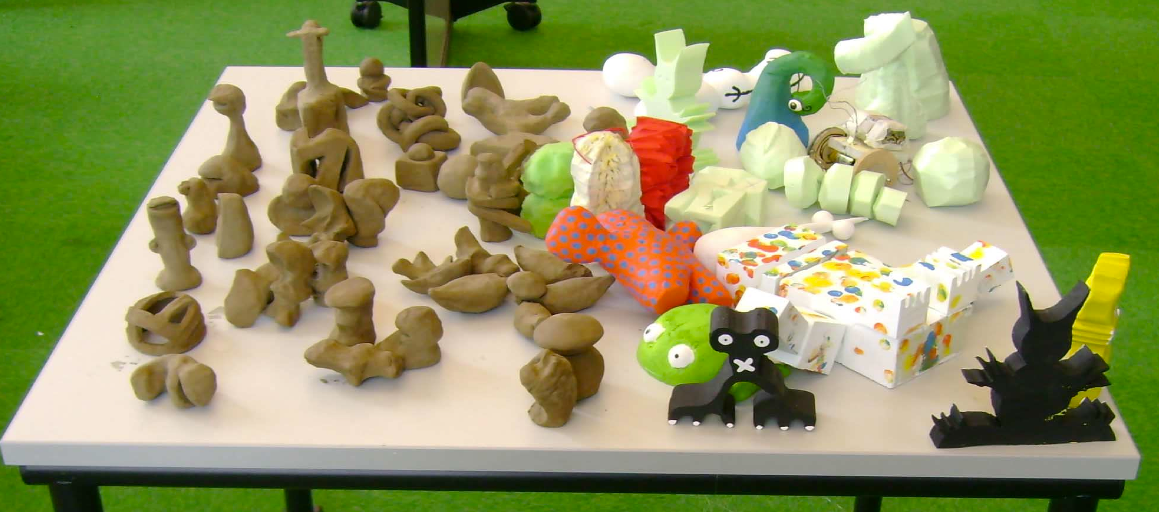
\includegraphics[width=\linewidth]{gfx/vyasModelle}}
	\end{center}
		\caption[Physikalische Modelle. \newline \citep{Vyas:2008}]{Einige physikalische Modelle, erstellt in einem Designstudio.}\label{fig:vyasModelle}
\end{figure}

\begin{quote}
	\textsl{>>One thing that we know is that sketches for experience and interaction desgin will likely differ from conventional sketching since they have to deal with time, phrasing, and feel - all attributes of the overall user experience.<<}
\begin{flushright}\citep{Buxton:2007}\end{flushright}
\end{quote}

Auch wenn sich \emph{Sketches for Experience} von herkömmlichen Skizzen unterscheiden, unterliegen sie trotzdem denselben Eigenschaften.

\medskip Skizzen sollten:
\begin{itemize}
	\item Schnell, reichlich und in kurzer Zeit herstellbar, billig und verwerfbar sein,
	\item Eindeutige Gestik, minimale Detailstufe und angemessenen Grad an Feinheit haben,
	\item und durch Mehrdeutigkeit zum Erforschen und Vorschlagen anregen.
\end{itemize}
\begin{flushright}\citep{Buxton:2007}\end{flushright}

\subsubsection{Low-fidelity Prototypen} \index{Prototyping!Low-fidelity} Skizzen werden auch öfters fälschlicherweise als Prototypen angesehen. Da im nächsten Punkt näher auf Prototypen eingegangen wird, soll an dieser Stelle lediglich auf die Eigenschaften von \emph{Low-fidelity Prototypen}, welche Skizzen am ähnlichsten sind, Bezug genommen und der Unterschied zu Skizzen verdeutlicht werden.

\medskip \emph{Low-fidelity Prototypen} haben wie Skizzen wenig Ähnlichkeit mit fertigen Produkten. Es werden Materialien, wie z.B. Papier oder Karton verwendet, die sich von der gewollten fertigen Version unterscheiden. Sie sind simpel, billig in der Herstellung und leicht zu verändern. \emph{Low-fidelity Prototypen} werden nie mit dem Hintergedanken produziert sie zu behalten und in das Endprodukt zu integrieren \citep{Sharp:2002}.

\medskip Trotz der Ähnlichkeit zu Skizzen, besteht ein feiner Unterschied. Beide beschreiben zwar Designkonzepte, dienen aber unterschiedlichen Zwecken und finden folglich in verschiedenen Stadien des Designprozesses Einsatz. Skizzen werden wie schon erwähnt in den anfänglichen Phasen	der	Ideenfindung verwendet, wobei Prototypen im	Allgemeinen	erst in späteren Phasen eingesetzt werden. Wie \autoref{fig:sagmeisterElaborationReductionFunnels} zeigt, können \emph{Sketching} und \emph{Prototyping} als Trichter im Design Prozess verstanden werden. Am Anfang des Prozesses steht die Ausarbeitung verschiedenster Ideen und Möglichkeiten – am Ende die Reduzierung dieser bzw. die Entscheidungsfindung.
Ebenfalls unterscheidet sich der Aufwand beider Methoden, da Prototypen im Gegensatz zu Skizzen mehr Zeit benötigen bis sie fertig gestellt sind. Sie besitzen somit auch nicht den Wegwerfcharakter einer Skizze. \\
Der Unterschied liegt also nicht in	der	Form der Methoden, sondern eher im Nutzen bzw. in der Bedeutung dieser,	welcher	durch fließende Übergänge beider Methoden in \autoref{fig:buxtonSketch2prototype} anschaulich dargestellt wird \citep{Sagmeister:2008}.

\medskip Per Definition ist eine Skizze ein grobes, ungefähres Design. Es ist lückenhaft, mangelhaft und hat unausgereifte Eigenschaften. Im Gegensatz dazu hilft ein Prototyp Ideen auszuwerten - entweder durch Absprache mit dem Klienten, in der sie ihn ausprobieren, oder durch Usabilitytests. Nicht überraschend, können vorzeitige Usabilityauswertungen von Skizzen bzw. Prototypen, signifikante Probleme aufzeigen, die das Design frühzeitig vernichten - vorallem wenn neue Designs mit konservativeren verglichen werden. Das zieht Folgen für die Entwickler und Forscher mit sich \citep{Greenberg:2008}.
	
\begin{figure}
	\begin{center}
        {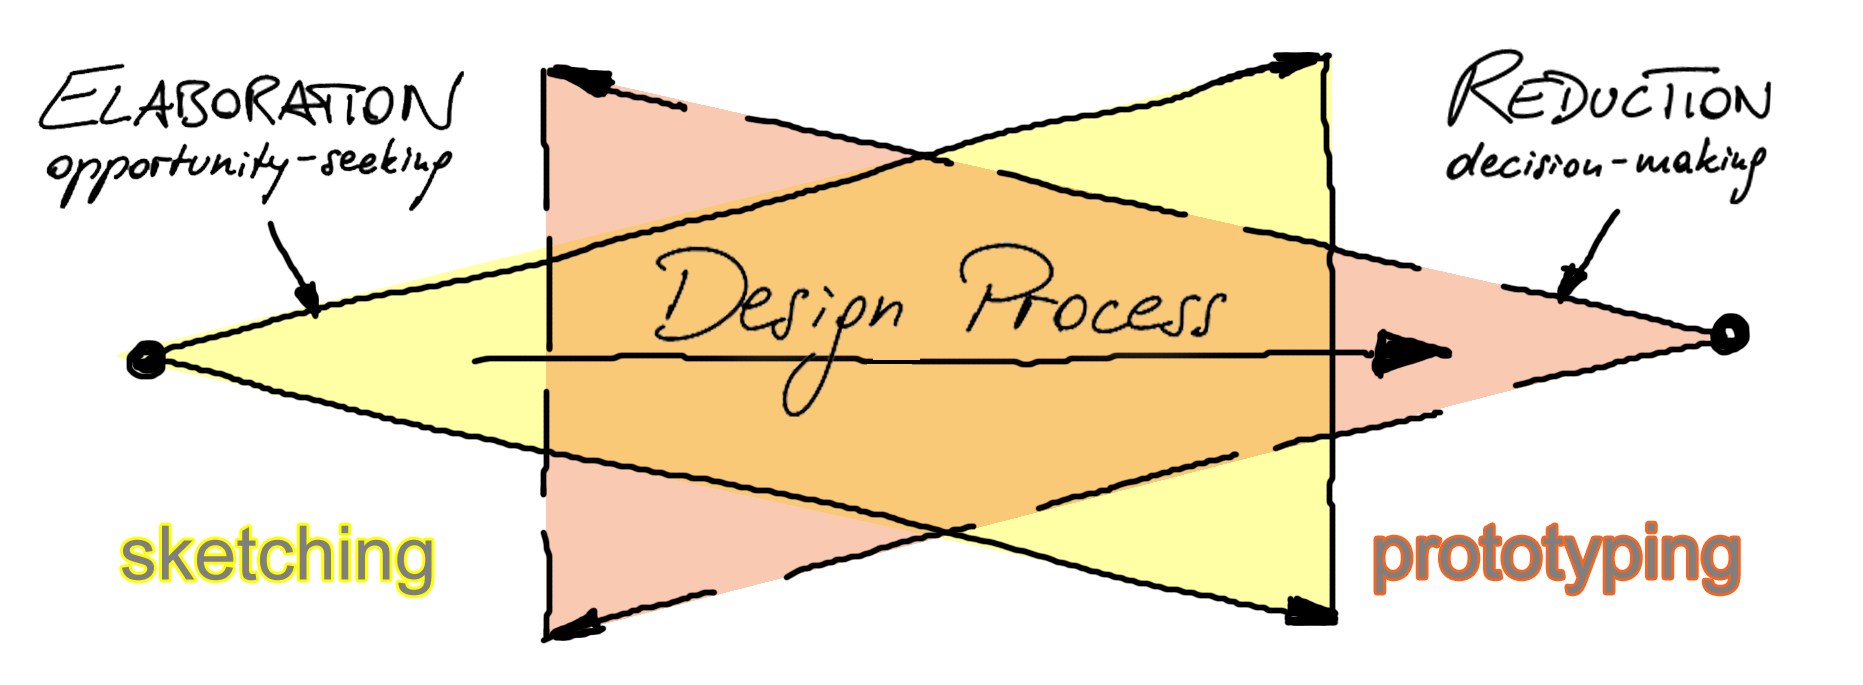
\includegraphics[width=\linewidth]{gfx/sagmeisterElaborationReductionFunnels}}
	\end{center}
		\caption[Skizzen und Prototpyen im Designprozess. \newline \citep{Sagmeister:2008}]{Skizzen und Prototpyen im Designprozess. Die Reduktion, die durch Entscheidungsfindungen bei Prototypen entsteht, wird durch Ausarbeitung von neuen Ideen mit Skizzen ausgeglichen. Dies verdeutlicht die Bedeutungen beider Methoden und deren Einsatzzweck.}\label{fig:sagmeisterElaborationReductionFunnels}
\end{figure}

\begin{figure}
	\begin{center}
        {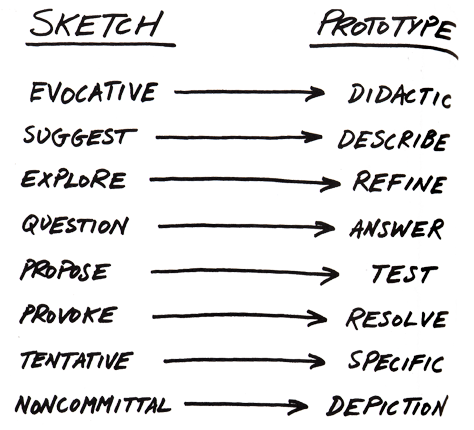
\includegraphics[width=\linewidth]{gfx/buxtonSketch2prototype}}
	\end{center}
		\caption[Übergang von Skizzen zu Prototypen. \newline \citep{Buxton:2007}]{Übergang von Skizzen zu Prototypen. Der Unterschied von Skizzen und Prototypen liegt nicht in der Form der Methoden sondern im Nutzen bzw. in der Bedeutung. Die Pfeile zeigen, dass es sich hierbei um einen fließenden Übergang handelt.}\label{fig:buxtonSketch2prototype}
\end{figure}
\clearpage

\subsubsection{Getting the Right Design vs. Getting the Design Right} \index{Design!getting it right} \label{sssec:rightDesign}
Die Kehrseite frühzeitiger Usability Auswertungen von Skizzen animieren Entwickler jedes Problem in iterativen Schritten zu lösen. Das führt zu >>local hill climbing<<, in dem viel Aufwand betrieben wird um das anfängliche Design richtig hinzubekommen (\emph{Getting the Design Right}) (siehe \hyperref[fig:greenbergBuxtonRightDesign]{Abbildung \ref{fig:greenbergBuxtonRightDesign}a}). Unglücklicherweise blockieren Auswertungen früher Skizzen, Designer oft davon andere, vielleicht bessere Ideen zu entwickeln. \citep{Greenberg:2008}

\medskip Eine Skizze bildet typischerweise nur eines der möglichen Designs und Variationen zum Abwägen ab. Frühes Design benötigt jedoch viele Ideenskizzen, einen Vergleich vieler konkurrierender Ideen und eine Auswahl des aussichtsvollsten Designs (siehe \hyperref[fig:greenbergBuxtonDesignRight]{Abbildung \ref{fig:greenbergBuxtonDesignRight}}). Die aussichtsvolle Idee wird dann weiter abgestimmt und entwickelt, bis man sie als Prototyp verwenden kann. In anderen Worten: Skizzieren dreht sich um das Finden des richtigen Designs (\emph{Getting the Right Design}) \citep{Tohidi:2006, Buxton:2007, Greenberg:2008}. 

\begin{figure}
	\myfloatalign
	\subfloat[Getting the Right Design.]
	{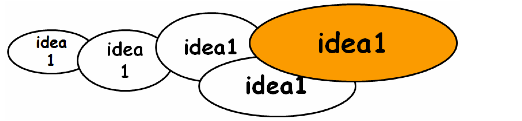
\includegraphics[width=\linewidth]{gfx/greenbergBuxtonDesignRight}} \\
	\subfloat[Getting the Design Right.]
	{\label{fig:greenbergBuxtonDesignRight}%
	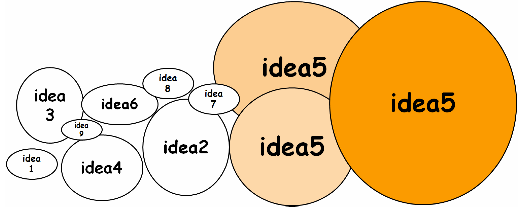
\includegraphics[width=\linewidth]{gfx/greenbergBuxtonRightDesign}} \\
	\caption[Getting the Right Design vs. Getting the Design Right. \newline \citep{Greenberg:2008}]{Getting the Right Design vs. Getting the Design Right. Die richtige Herangehensweise ist das Erstellen von Skizzen, danach das iterative Design, gefolgt von Auswertungen.}\label{fig:greenbergBuxtonRightDesign}
\end{figure}

\subsection{Prototyping} \index{Prototyping}
Der abschließende und wichtigste Schritt bevor ein Produkt oder Service engeführt, oder idealerweise mit Benutzern getestet wird, ist die Erstellung eines Prototyps - oder besser mehrerer Prototypen.

\begin{quote}
	\textsl{>>Prototyping is where, finaly, all pieces of the design come together in a holistic unit.<<}
\begin{flushright}\citep{Saffer:2007}\end{flushright}
\end{quote}

Viele Auftraggeber haben Schwierigkeiten ein Design zu verstehen, bevor sie nicht einen Prototypen gesehen und benutzt haben. Prototypen sind ein Kommunikationswerkzeug. Sie übermitteln die Botschaft >>So könnte das Ganze aussehen und funktionieren<<.

\medskip Industrial Designer z.B. erstellen in dieser Phase ein glaubwürdiges Modell eines Produktgehäuses, einschließlich Knöpfe, Drehschalter oder anderer Bauteile, welches so real aussieht, dass es sogar die Auftraggeber täuschen kann. Zusätzlich werden oft Screen Designs, Animationen oder interaktive Demonstrationen erstellt, um Benutzern zu zeigen, wie das Produkt reagieren soll \citep{Vertelney:1990}.

\medskip Welche Form aber nun Prototypen im Allgemeinen annehmen, hängt von den Mitteln ab, die Designern zu Verfügung stehen bzw. von der Art des Produkts um das es sich handelt. Ein Designer mit den richtigen Ressourcen kann \emph{high-fidelity Prototypen} erstellen, welche so aussehen und reagieren als wären sie das fertige Produkt.

Der Zweck von Prototypen ist aber das Erforschen der Eigenschaften des Endprodukts. Ein Prototyp ist vielleicht effizient und ausdruckslos und ein anderer ist wiederum skurril und zugänglich. Der eine ist Menü-basiert und der andere benutzt direkte Manipulationen. Designer benutzen Prototypen um herauszufinden, welche Funktionen oder Eigenschaften funktionieren, und zwar für sich selbst, die Auftraggeber und die Benutzer \citep{Saffer:2007}. Da Designer nicht unfehlbar sind und somit das erste Design nicht perfekt sein wird, werden die Erkenntnisse, welche aus diesen sog. \emph{>>formative Evaluations<<} gewonnen werden, zur Erstellung verbesserter Prototypen benutzt. Dieser iterative Prozess aus Verbesserungen läuft so lange bis klarer weise keine Verbesserungen mehr nötig sind. Oder mit anderen Worten: 

\begin{quote}
	\textsl{>>This is exactly how iterative prototyping works: you start somewhere, evaluate it to see how to make it better, change it to make it better and then keep on doing this until it can't get any better.<<}
\begin{flushright}\citep{Dix:2004}\end{flushright}
\end{quote}

Eine Gefahr, die Prototyping mit sich bringen kann, ist die Wahl eines falschen Anfangsdesigns. Wenn man mit einem schlechten Design-Konzept beginnt Prototypen zu erstellen, kann es sein, dass man am Ende nur eine >>verschönerte<< Version der schlechten Idee bekommt (vgl. \ref{sssec:rightDesign} \nameref{sssec:rightDesign}).\\ Die Vorraussetzungen um Prototyping Methoden richtig einsetzen zu können sind also:

\begin{enumerate}
	\item Ein Verständnis über die Elemente die neu designed gehören und wie man sie verbessern kann, und
	\item Ein gutes Anfangsdesign als Startprodukt.
\end{enumerate}
\begin{flushright}\citep{Dix:2004}\end{flushright}

Gute Designer schaffen es vielleicht auch durch Erfahrung und Urteilungsvermögen ein passendes Anfangsdesign zu finden, jedoch wird auch ihnen dies durch die Komplexität der Probleme, gerade in Interaction Design, erschwert. Das Ausarbeiten von Skizzen und Modellen, um Probleme aus verschiedenen Blickwinkeln zu beleuchten ist deswegen gerade vor dem Erstellen von Prototypen essenziell.
Die meisten Designer arbeiten mit drei Arten von Prototypen: Digitalen Prototypen, physikalischen Prototypen und Prototypen aus Papier. Es soll nun kurz näher auf diese eingegangen und im Besonderen \emph{Paper Prototyping} diskutiert werden. 

\subsubsection{Digitale Prototypen} \index{Prototyping!Digital}
Digitale Prototypen (siehe \autoref{fig:safferDigitalPrototype}) können verschiedenste Formen annehmen, von statischen Bildern bis hin zu komplexen 3D Umgebungen. Sie können in ihrer Funktionalität sehr eingeschränkt sein – z.B. indem sich Benutzer durch eine Reihe an Bildern >>durchklicken<< - oder im hohen Grade funktionell, so dass User in der Lage sind mit dem System zu arbeiten als wäre es das Endprodukt. Entscheidet man sich für die komplexere Variante, sollten reichhaltig Funktionen vorhanden sein, um das problemlose Interagieren des Users gewährleisten zu können. Es ist schwer für Benutzer sich z.B. ein Werkzeug um Rechtecke zu zeichnen vorzustellen, ohne es dabei wirklich benutzen zu können. Die Gefahr dabei ist jedoch, dass Benutzer und Auftraggeber denken könnten, dass der Prototyp bereits das finale Produkt ist. Fügt man einmal ein visuelles Design hinzu, richtet man seine Aufmerksamkeit diesem anstatt auf die Funktionalität \citep{Saffer:2007}.\\
Seit den 80er Jahren gibt es für beide Formen digitaler Prototypen eine Vielfalt an Programmen zur Erstellung dieser. Seien es Programme wie \emph{MacDraw}, \emph{Protoscreens}, oder \emph{Prototyper} damals, oder Tools wie \emph{Photoshop}, \emph{Shockwave} oder \emph{Visual Basic} heutzutage; sie alle verfügen über die Funktionalität, Prototypen (mit ihren beschränkten Grad an Nutzen) zu erstellen \citep{Miller-Jacobs:1991}. \\
Ein Vorteil der daraus entsteht, ist dass digitale Prototypen leicht veröffentlicht werden können. Designer können sie einfach aufs Web stellen oder auf Disks verbreiten, um Benutzern die Möglichkeit zu bieten, die Prototypen egal wo sie sind auszuprobieren. 

\begin{figure}
	\begin{center}
        {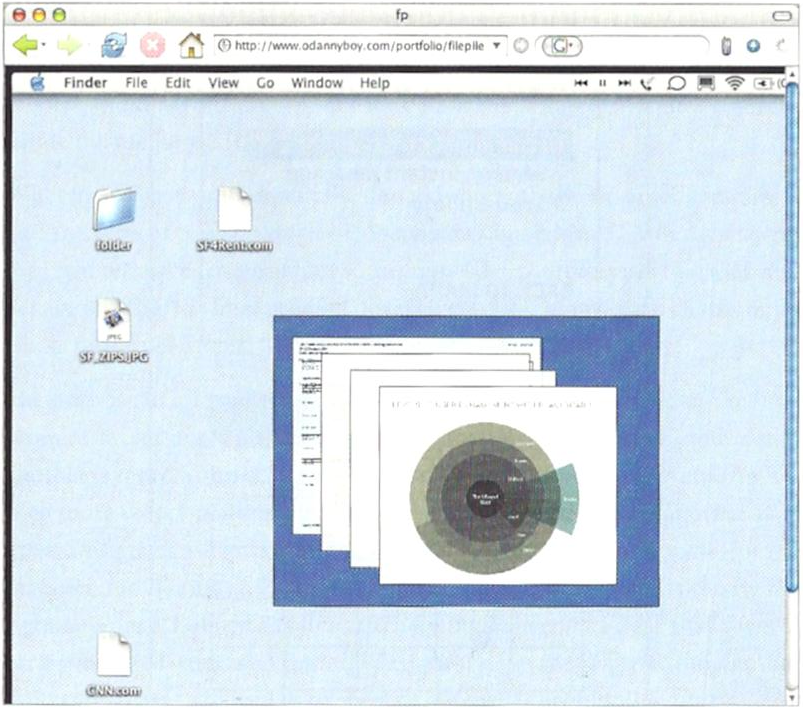
\includegraphics[width=\linewidth]{gfx/safferDigitalPrototype}}
	\end{center}
		\caption[Digitale Prototypen. \newline \citep{Saffer:2007}]{Digitale Prototypen können Formen in verschiedener Detailstufen annehmen und leicht über das Internet verbreitet werden.}\label{fig:safferDigitalPrototype}
\end{figure}

\subsubsection{Physikalische Prototypen} \index{Prototyping!Physikalisch}
Physikalische Prototypen (siehe \autoref{fig:safferPhysicalPrototype}) können simple Teile eines Designs (wie zum Beispiel einzelne Schalter oder Wahltasten) bis hin zu kompletten physikalischen Umgebungen schaffen. Wie aber auch bei anderen Prototypen kann sich dabei die Funktionalität und Beschaffenheit unterscheiden. Ein Gerät beispielsweise kann aus exakt denselben Materialien wie das Endprodukt erstellt werden (z.B. Plastik oder Metall), oder durch Materialien wie Holz oder Ton angeglichen werden. 

\begin{figure}
	\begin{center}
        {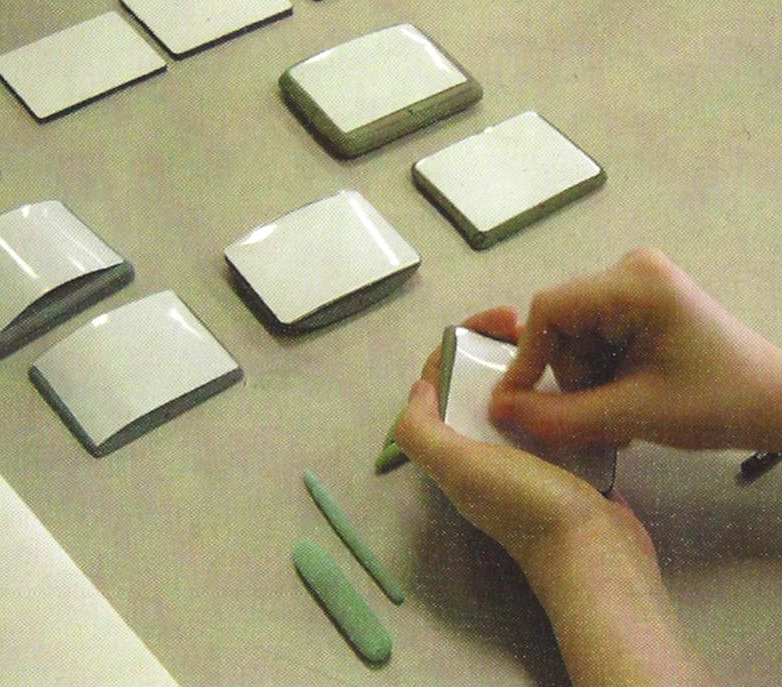
\includegraphics[width=.8\linewidth]{gfx/safferPhysicalPrototype}}
	\end{center}
		\caption[Physikalische Prototypen. \newline \citep{Saffer:2007}]{Physikalische Prototypen können so klein wie ein Schalter sein, oder so groß wie ein ganzer Raum.}\label{fig:safferPhysicalPrototype}
\end{figure}

\subsubsection{Papier Prototypen} \index{Prototyping!Papier}
Papier Prototypen sind meistens die schnellste Art um die Funktionalität eines Produkts oder Services zu demonstrieren. Vor allem im Interaction Design kann ein Designer auf Papier leicht einen gesamten Systemdurchlauf erstellen, wobei jedes Blatt Papier einen ‚Moment’ des Designs repräsentiert. Diese Momente könnten eine Webseite, ein Screenshot oder Teil eines Services sein. Zuseher können so Schritt für Schritt den Prototyp durchlaufen indem sie sich in einer gewissen Reihenfolge zwischen den Seiten bewegen.
Wie diese Bewegung abläuft, kann auf mehrere Arten erfolgen. Dan Saffer z.B. schlägt vor die Seiten zu nummerieren, und dem User klare Instruktionen zu geben wie er vorzugehen hat („Wenn Sie diesen Button drücken, gehen Sie auf Seite 9“). Während des Testens können bei diesem Verfahren Beteiligte, also Benutzer und Designer, Kommentare und Notizen direkt auf dem Prototyp schreiben \citep{Saffer:2007}.\\
Carolyn Snyder hingegen vertritt eine andere Auffassung von \emph{Paper Prototyping}: 

\begin{quote}
	\textsl{>>Paper prototyping is a variation of usability testing where representative users perform realistic tasks by interacting with a paper version of the interface that is manipulated by a person "playing computer", who doesn't explain how the interface is intended to work.<<}
\begin{flushright}\citep{Snyder:2003}\end{flushright}
\end{quote}

Laut ihr hat mindestens eine Person neben dem User zu sitzen und agiert (vollkommen still) als Computer und übernimmt dessen Aufgaben. Kommentare und Notizen machen andere Personen, die ebenfalls still als Beobachter im Raum sitzen. Zusätzlich kann noch ein Moderator hinzu gezogen werden, welcher dem User das Umfeld erklärt bzw. ihm Aufgabenstellungen erteilt.

\medskip Im Allgemeinen signalisieren Papier Prototypen, egal nach welcher Methode erstellt, den Benutzern, dass es sich hierbei noch nicht um das Endprodukt handelt und gewähren ihnen somit unterbewusst mehr Freiheiten, Eigenschaften und Funktionsweisen zu kommentieren. Snyder fasst weiters folgende Vorteile zusammen:

\medskip Papier Prototypen:
\begin{itemize}
	\item Liefern substanzielles User Feedback in einem frühem Stadium des Entwicklungsprozesses (bevor Bemühungen in die Implementierung gesteckt wurden),
	\item Fördern schnelle iterative Entwicklung, durch Experimente mit mehreren Ideen, anstatt nur mit einer,
	\item Erleichtern die Kommunikation innerhalb des Entwicklungsteams sowie zwischen dem Team und den Benutzern,
	\item Erfordern keine technischen Fähigkeiten, womit eine multidisziplinäre Mannschaft zusammenarbeiten kann, und
	\item Regen Kreativität im Produktentwicklungsprozess an.
\end{itemize}
\begin{flushright}\citep{Snyder:2003}\end{flushright}
	
Paper Prototyping folgt somit dem >>Maximum Feedback for Minimum Effort<< - Prinzip. Wie sieht aber nun ein Papier Prototyp aus und wie wird er erstellt?

\medskip Materialien wie einfaches weißes Papier, unlinierte Karteikarten, Marker, Stifte, Scheren, durchsichtiges entfernbares Klebeband, transparente Folien, Permanentmarker usw. dienen als Werkzeuge in Paper Prototyping.\\
Durch sie werden anfangs Hintergründe bzw.  Hintergrundsmasken\index{Hintergrundsmasken} kreiert. Diese können z.B. gezeichnete Repräsentationen eines Browserfensters sein, wenn der Browser mit seinen herkömmlichen Funktionen über den Testverlauf hinweg unverändert bleibt, oder andere statische Gegebenheiten. Ein Hintergrund ist zwar nicht immer notwendig, zeigt dem Benutzer jedoch, dass er es mit einer Repräsentation eines Computerbildschirms oder anderen elektronischen Gerät zu tun hat und sich somit auf diese konzentrieren soll. Es kann manchmal auch helfen - besonders bei kleinen Geräten (z.B. bei PDAs oder Handys) – durch Masken den nutzbaren Platz zu begrenzen, da gerade hier oft jeder Pixel zählt. \autoref{fig:snyderMasks} zeigt dazu ein Beispiel. \\
Nachdem die Hintergründe bzw. Masken\index{Masken|see{Hintergrundsmasken}} erstellt wurden, ist es nötig alle Interface Widges, wie \emph{buttons}, \emph{checkboxes}, \emph{dialog boxes}, \emph{text fields}, \emph{lists}, \emph{cursors} etc. zu erstellen. Interface Widges helfen später im User Testing die Interaktivität zu simulieren \citep{Snyder:2003}.

\begin{figure}
	\begin{center}
        {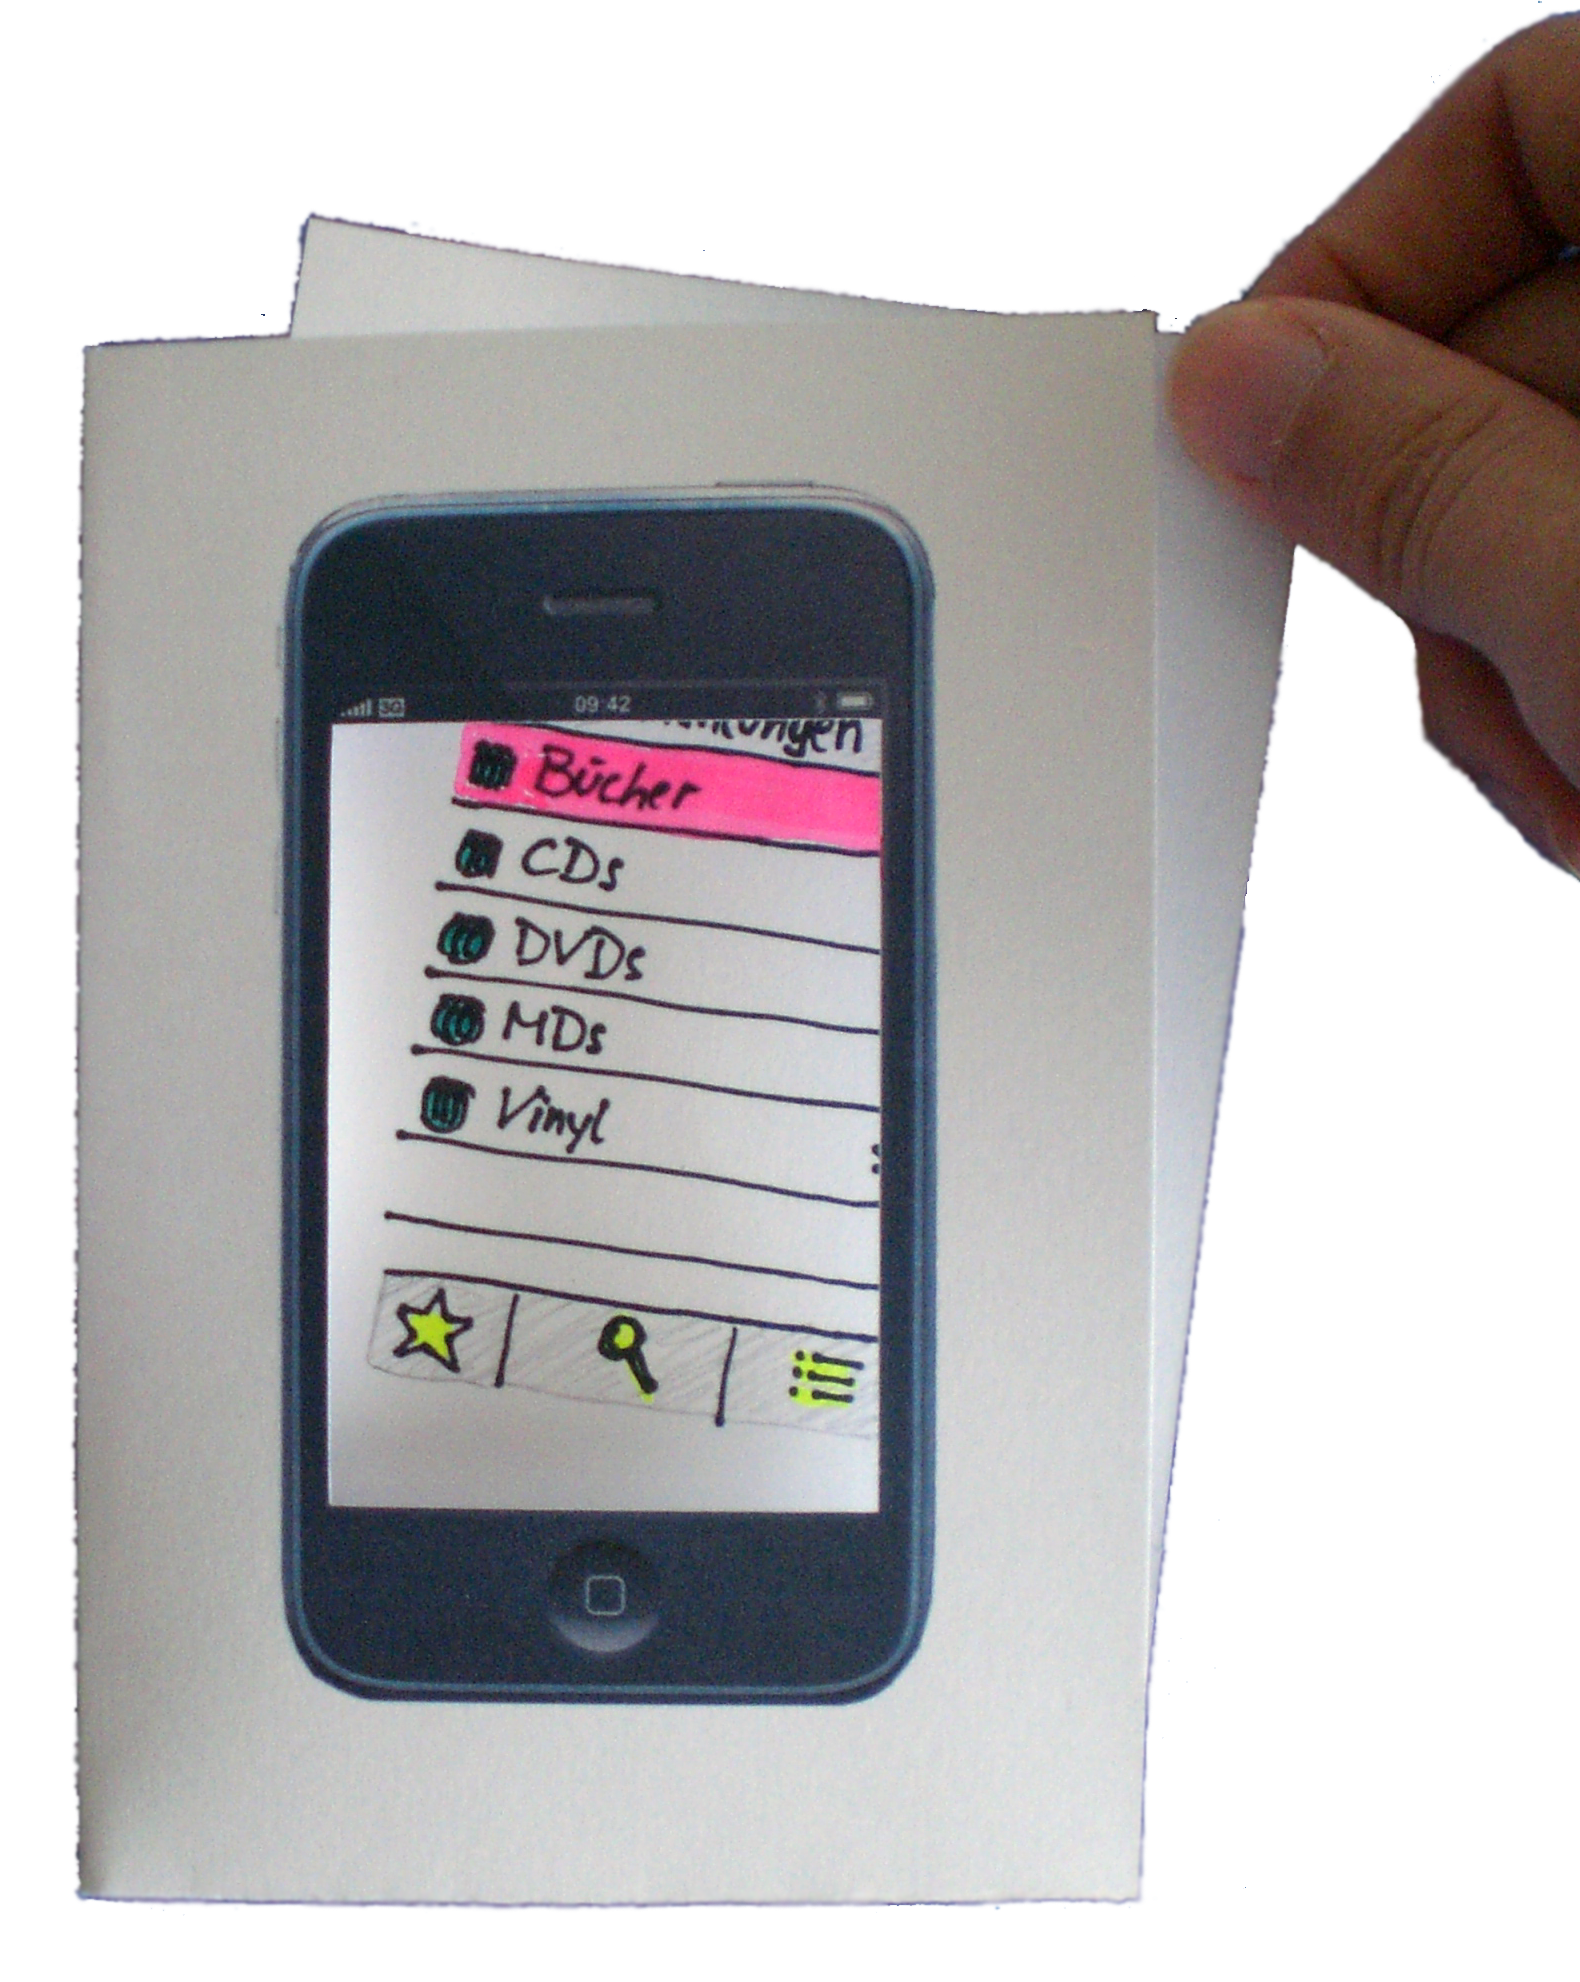
\includegraphics[width=.7\linewidth]{gfx/snyderMasks}}
	\end{center}
		\caption[Hintergrundmasken \newline \citep{Snyder:2003}]{Hintergrundmasken werden im ersten Schritt von Paper Prototyping erstellt. Besonders bei kleinen Geräten kann es helfen, den nutzbaren Bereich einzugrenzen, da hier meist jeder Pixel zählt.}\label{fig:snyderMasks}
\end{figure}

\medskip Sie sollten deswegen so gut wie möglich vorbereitet werden, um lange Wartezeiten im Testing zu vermeiden. Im Allgemeinen ist es natürlich auch erlaubt Screenshots von Elementen (inklusive Hintergrund) zu machen, jedoch muss man sich dabei immer fragen wie viel man vielleicht nachträglich ändern will. Meistens ist es schneller, Elemente selbst zu zeichnen. \autoref{fig:snyderPaperPrototype} zeigt Vorbereitungselemente aus den verschiedensten Materialien und deren möglichen Einsatzzweck \citep{Snyder:2003}.

\begin{figure}
	\myfloatalign
	\subfloat[Papierelemente]
	{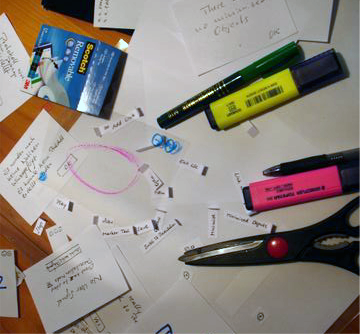
\includegraphics[width=.48\linewidth]{gfx/snyderPaperElements}} \quad
	\subfloat[Papier Prototyp]
	{\label{fig:snyderPaperElements}%
	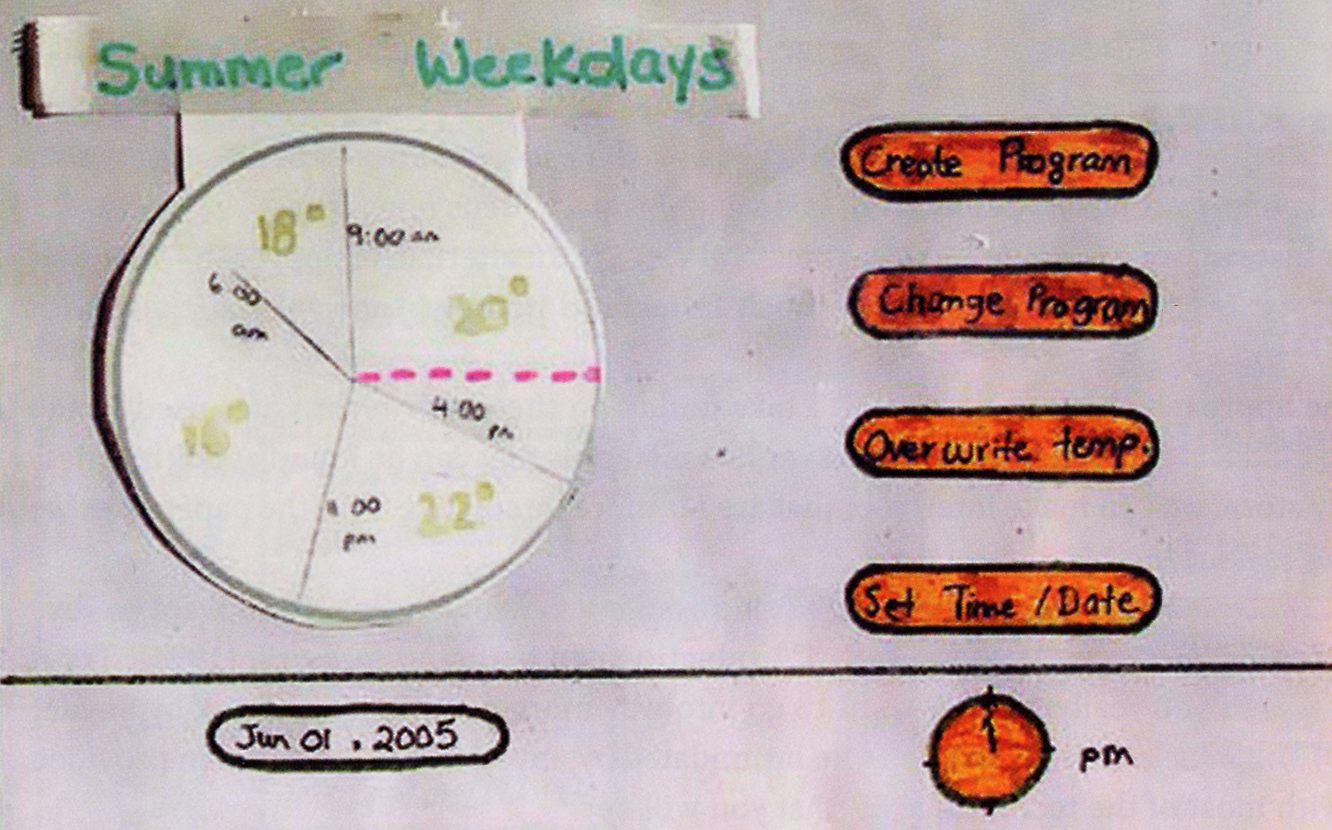
\includegraphics[width=.48\linewidth]{gfx/snyderPaperPrototype}} \\
	\caption[Paper Prototyping \newline \citep{Sagmeister:2008}]{Papierelemente (a) für Interface Widges können durch einfache Materialien wie Papier und Stifte erstellt werden. Sie sollten vor dem User Testing vorbereitet werden, um lange Wartezeiten zu vermeiden. Ein Papier Prototyp, wie in (b), imitiert zwar nur das Enprodukt, bietet dem User aber die volle Interaktivität. Der Benutzer interagiert dabei direkt mit dem Prototypen als wäre es ein Touch Screen.}\label{fig:snyderPaperPrototype}
\end{figure}

\medskip Nachdem ein Prototyp fertig gestellt wurde, sollte er logischerweise auch Einsatz finden. Das richtige Publikum dafür sind die User, die das Endprodukt benutzen werden. Man nennt diesen Prozess auch User Testing, der im folgenden Punkt beschrieben wird.

\subsection{(User) Testing} \index{Testing} \index{User Testing|see{Testing}}
Der oft verwendete Begriff User Testing ist eigentlich eine Fehlbezeichnung. Getestet werden natürlich nicht die User sondern das Produkt bzw. das Service. 
Das Testen mit potentiellen Benutzern hilft falsche Annahmen, die in der Vorbereitung bzw. Erstellung des Designs gemacht wurden, zu korrigieren. Am besten werden diese durch Beobachtungen und Rücksprache mit den Testpersonen aufgedeckt. Dabei ist es oft am besten, wenn Designer anderen Teammitgliedern oder \emph{Usability Spezialisten} gestatten die Tests zu leiten, um selbst eine Beobachterrolle einzunehmen. Designer neigen meist dazu ihr Gegenüber zu belehren (>>Schau doch mal zu den Button rechts oben<<), weil sie ihr Design besser kennen. Es sollte zusätzlich vermieden werden, dass sich Designer als solche zu erkennen geben, da Testpersonen oft ihr Feedback danach richten bzw. gegebenenfalls ihre Kritik abschwächen. Auch wenn für Designer nichts demütigender ist, als anzusehen wie Testpersonen durch ihr Design stolpern, müssen sie diese Bürde auf sich nehmen, die Testdurchläufe ernst nehmen und nach Verhaltensmustern Ausschau halten.  Diese bewegen sie dann dazu, Prototypen zu ändern und sie erneut zu testen. Erfahrene Designer wissen eins mit Sicherheit: Das erste Design ist es selten das richtige. \\
Testings werden am besten direkt im geplanten Umfeld der Endnutzer durchgeführt, es sei denn ein handelt sich um ein Service, dass eine bestimmte Prototypumgebung erfordert. Digitale und physikalische Prototypen sollten somit auf ihren geplanten Computern und Umfeldern Anwendung finden (vgl. \autoref{fig:safferUserTesting}). Papier Prototypen erfordern eine bestimmte Prototyp-umgebung, die es erlaubt die Testings auch in Testlaboratorien o.ä. durchzuführen. Testlaboratorien haben den Vorteil, dass Designer viele Tests an einem einzigen Tag durchführen können, ohne dabei den Ort wechseln zu müssen \citep{Saffer:2007}.

\medskip Je nach Qualität bzw. Aufwand der für einen Prototypen betrieben wurde, variiert auch der Ablauf eines User Testings. Oft reicht es, wie z.B. bei \emph{high fidelity} Digitalprototypen, dem User lediglich eine Aufgabe zu stellen und ihn dann sich selbst zu überlassen um ihn zu beobachten. Manchmal benötigt man auch einen Moderator, der den User durch den Testablauf leitet. Bei \emph{low fidelity} Prototypen jedoch, zu denen meist Papierprototypen zählen, muss mehr Aufwand betrieben werden. Wie schon im vorigen Punkt erwähnt, ist es notwendig jemanden den Part des Computers bzw. Gerätes übernehmen zu lassen. Bei Paper Prototyping sitzt diese Person meist neben oder gegenüber der Testperson und übernimmt stillschweigend alle interaktiven Tätigkeiten.

\medskip Dieses Prinzip ist aber nicht nur eine Eigenheit von Papierprototypen. Eine der ersten Anwendungen fand sich schon 1971 mit dem Testen eines elektronischen Flugticket Schalters am Chicago O’Hare Airport \citep{Erdmann:1971}. Da es von echten Kunden, mit echtem Geld zur Anschaffung echter Tickets für damals aktuelle Flüge verwendet wurde, musste es nicht nur von der \emph{user-interaction}-Perspektive, sondern auch von der organisatorischen und finanziellen Seite her arbeiten. Doch da das System noch nicht fertig gestellt war und man es trotzdem einem Test unterziehen wollte, musste eine Person im Hintergrund alle Tätigkeiten, wie am normalen Ticketschalter, managen. Auch wenn es aus Sicht des Kundenservices teuer und ineffizient schien, brachte es wichtige Informationen über das Desgin, die \emph{Usability} und die Akzeptanz mit sich \citep{Buxton:2007}.

\begin{figure}
	\begin{center}
        {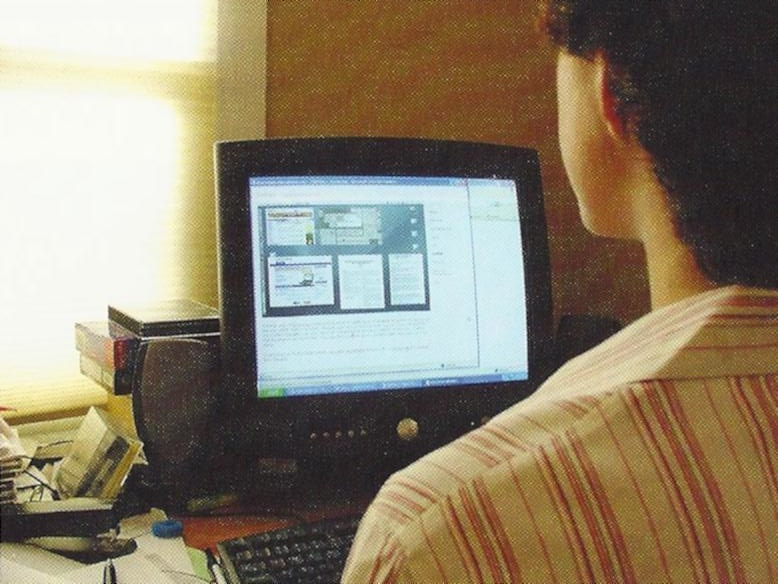
\includegraphics[width=\linewidth]{gfx/safferUserTesting}}
	\end{center}
		\caption[(User) Testing \newline \citep{Saffer:2007}]{Testings werden am besten im geplanten Umfeld der Endnutzer durchgeführt. Ein digitaler Prototyp sollte z.B. beim Benutzer zu Hause getestet werden.}\label{fig:safferUserTesting}
\end{figure}

\begin{figure}
	\begin{center}
        {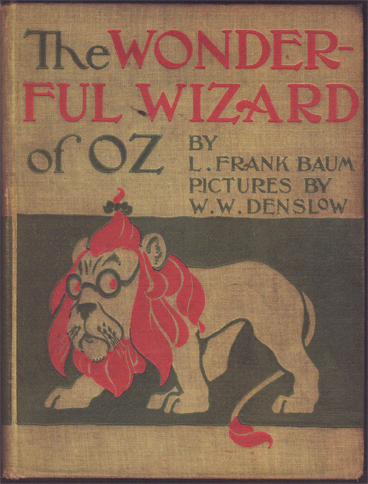
\includegraphics[width=\linewidth]{gfx/buxtonWizardOz}}
	\end{center}
		\caption[Wizard of Oz \newline \citep{Buxton:2007}]{Das Cover der Erstedition des Buches, das einen unerwarteten Einfluss auf das Thema Interaction Design zur Folge hatte. Die Wizard of Oz Technik beschreibt eine Interaktion zwischen Mensch und Maschine in der eine Person die Reaktionen eines Systems erzeugt.}\label{fig:buxtonWizardOz}
\end{figure}

\medskip Diese Art des Testens nennt man auch \emph{Wizard of Oz Technique}\index{Wizard of Oz Technique}, die ihren Ursprung in der Kindergeschichte \emph{The Wonderful Wizard of Oz} von L. Frank Baum findet. (siehe \autoref{fig:buxtonWizardOz}) \\ Sie handelt von einem kleinen Mädchen Dorothy, welches zusammen mit ihrem Hund Toto von einem Wirbelsturm von ihrer Farm in Kansas in das Land der Munchkins getragen wird. Verzweifelt, mit dem Wunsch wieder nach Hause zu kommen, traf sie auf die Gute Hexe des Nordens, die der gelandeten Dorothy riet, in die Smaragdstadt zu gehen und dort den Zauberer von Oz um Hilfe zu bitten. Mit neu gefunden Freunden zog Dorothy los und fand tatsächlich den Zauberer, der sich jedem in einer anderen Gestalt zeigte. Er versicherte zu helfen, unter der Bedingung, dass einer die Böse Hexe des Westens tötet. Nach einigen Abenteuern schafften sie dies auch und kehrten zurück zum Zauberer um das Versprechen, das er ihnen gab einzulösen. Nach anfänglichem Zögern seitens des Zauberers von Oz, sich zu zeigen, brachten sie ihn schlussendlich dazu und mussten feststellen, dass er gar kein großer Zauberer war, sondern nur ein alter Mann, den durch seine Ankunft mit einem Heißluftballon jeder als Magier ansah. \citep{Baum:2008}

\medskip Dorothy und ihr Hund Toto fanden natürlich einen anderen Weg nach Hause, die Geschichte zeigte uns aber, dass hinter dem großen \emph{Wizard of Oz} ein schüchterner alter Mann steckte, der mit seinem Trick so überzeugend war, dass er alle glauben ließ er sei jemand, der er gar nicht war. Und das ist auch die Quintessenz: 

\begin{quote}
	\textsl{>>To her the Wizard was real, and therefore so were all her experiences.<<}
\begin{flushright}\citep{Buxton:2007}\end{flushright}
\end{quote}

Folgt man also dem Beispiel des Zauberers, kann man im User Testing Systeme >>herbei beschwören<<, die den Benutzern reale wirkungsvolle Erfahrungen bieten, bevor das richtige System im eigentlichen Sinne existiert. Die wichtigsten Punkte, die man dabei beachten sollte sind folgende:

\medskip Eigenschaften von Testsystemen:\index{Testsysteme}
\begin{itemize}
	\item Es ist das Detailreichtum der Erfahrung und nicht die des Prototyps, Skizze oder Technologie, die wichtig ist, im Sinne der Ideenfindung und des Anfangsdesigns.
	\item Man kann alles verwenden, um diese Erfahrungen >>zu beschwören<<.
	\item Umso früher damit begonnen wird, desto wertvoller sind sie.
	\item Es ist einfacher, billiger, schneller und zuverlässiger einen alten Mann, ein Mikrofon und Lautsprecher zu finden als einen richtigen Zauberer. Dies gilt auch für die meisten Systeme:  Fake it before you build it.
\end{itemize}
\begin{flushright}\citep{Buxton:2007}\end{flushright}
	
Die Zielsetzung ist also nicht, das tatsächliche System zu bilden, sondern etwas nach zu ahmen, das Benutzer wirklich erfahren können. Das ermöglicht Design Konzepte in ihrer Tätigkeit zu erforschen und sie viel früher im Prozess zu erfahren als sonst möglich. Solch ein System sollte preiswert, schnell zu verwirklichen und verwerfbar sein und nur soviel Detailreichtum wie nötig besitzen, um seinen Zweck zu erfüllen. Es sollte somit alle Eigenschaften aufweisen, die auch Skizzen kennzeichnet, jedoch einer Regel unbedingt unterliegen: 

\begin{quote}
	\textsl{>>Generally the last thing that you should do when beginning to design an interactive system is write code.<<}
\begin{flushright}\citep{Buxton:2007}\end{flushright}
\end{quote}	

Mit den richtigen Testsystemen und klaren Aufgabenstellungen ist es für die Designer einfacher bestimmte Verhaltensmuster aus den Benutzererfahrungen zu erkennen. Oft werden zusätzlich im Laufe des Testings zu den vordefinierten Aufgaben, die Zeit und die Fehlerquote gemessen bzw. der Weg, wie ein User ein Problem löst, aufgezeichnet. Dies soll messbare Qualitätsmerkmale über das Design liefern und bei den abschließenden Rücksprachen mit den Benutzern Orientierungshilfe bieten.
Gewöhnlich werden 5-12 Testpersonen in ein Testing miteinbezogen. \citep{Dumas:1999} Meist sind es aber weniger, da man sich an einen fixen Projektzeitplan halten muss. Deswegen werden oft auch nur \emph{Quick and Dirty} – Tests mit 1-2 Usern durchgeführt, um schnelles Feedback zu einer Designidee zu bekommen \citep{Sharp:2002}.

\medskip Skizzieren, das Erstellen von Prototypen und Testen sind wichtige Methoden, um Ideen zu sammeln, sie zu einem Design zusammenzutragen und durch Erfahrungen zu verbessern bevor das endgültige Produkt erstellt wird. Viele Designer arbeiten mit ihnen effektiv und uneingeschränkt, jedoch ist es manchmal hilfreich zu wissen, von wem und wie genau ein Produkt verwendet werden soll. Dies wird nun abschließend im letzten Punkt erläutert.

\subsection{Personas \& Szenarien} \index{Personas} \index{Szenarien}

Der Begriff Personas umfasst eine Sammlung an typischen Personen, die mit einem Produkt oder Service zu tun haben. Sie zeigen Designern, dass sie für bestimmte Personen mit bestimmten Eigenschaften und Vorlieben designen und nicht schlicht für >>die Benutzer<<. 
Designer erfinden aus diesem Grund verschiedene Personas mit Hilfe von Beobachtungen und Unterhaltungen mit Usern. Zitate von diesen sind z.B. sehr nützlich, um Personas zu beschreiben (>>Ich fliege mindestens einmal pro Woche<<), oder um einfache Überschriften (>>Der häufige Passagier<<) zu finden. Personas fassen also Personen zusammen, die ähnliche Ziele, Beweggründe und Verhalten teilen. Ein Persona Dokument sollte diese Eigenschaften klar aufzeigen, um eine Persona von einer anderen unterscheiden zu können (siehe \autoref{fig:safferPersona}).

\begin{figure}
	\begin{center}
        {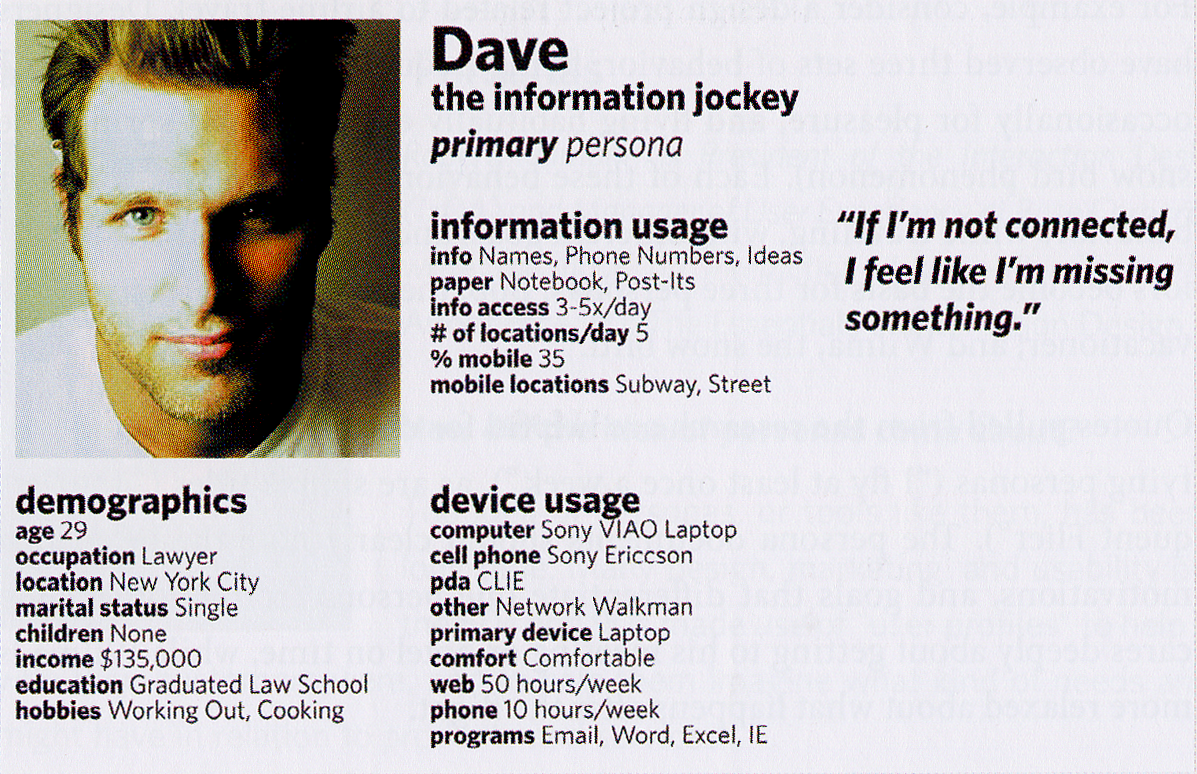
\includegraphics[width=\linewidth]{gfx/safferPersona}}
	\end{center}
		\caption[Persona \newline \citep{Saffer:2007}]{Personas verwandeln >>die Benutzer<< in identifizierbare menschliche Wesen.}\label{fig:safferPersona}
\end{figure}

\medskip Im Allgemeinen sollte man die Anzahl an Personas gering halten – am besten zwischen eins und sieben. Nach ca. sieben Personas fällt es einem schwer, sich an alle zu erinnern bzw. sie unterscheiden zu können. (vgl. \ref{ssec:GuidingPrinciples} \nameref{ssec:GuidingPrinciples}) Vor allem wird es mit zunehmender Anzahl immer schwieriger ein Design zu finden, welches allen Ansprüchen genügt. Man muss sich deswegen stets darum bemühen sich an das Kernverhalten zu richten, und nicht an alle verschiedenen Facetten.

\medskip Nachdem eine Sammlung an Personas zusammengestellt wurde, sollte man ein Foto für jede finden. Bilder helfen mehr als alles andere, eine persönliche Note hinzuzufügen und um sich leichter an diese zu erinnern. So lange Personas nicht veröffentlicht werden, können Fotos auch von Services wie z.B. \emph{Yahoo Personals} oder anderen Internetseiten verwendet werden. Personas an sich sind schlicht unbrauchbar wenn sie nicht zusammen mit Szenarien eingesetzt werden. In Szenarien können sie benutzt werden um Systemeigenschaften auf Nutzen und Eignung zu testen. 
Während viele Designer Personas nützlich finden, lehnen sie mache ganzheitlich ab. Diese Designer sehen Personas als eine Art künstliche Blockade zwischen dem Produkt und dessen Benutzer. Personas können jedoch, wenn sie auf Forschungen basieren und die richtigen Charakteristiken (Verhalten, Motivationen und Ziele) zeigen als wertvolles Tool dienen. Ob man Personas nun verwenden will, hängt schlussendlich vom Designer und der Größe des Projektes ab. \citep{Saffer:2007}

\medskip \emph{Szenarien} hingegen bieten einen schnellen und effektiven Weg um sich Design Konzepte vorzustellen. Man kann sie sich als Prototypen, welche lediglich aus Wörtern bestehen, vorstellen, da sie simple Geschichten bilden, welche fertig gestellte Produkte beschreiben. Die zentralen Darsteller dieser Geschichten sind Personas, die durch sie einen Kontext erhalten und zum Leben erwachen. Das Durchlaufen eines Szenarios mit verschiedenen Personas eignet sich somit perfekt zur Darstellung, Analyse und Planung der Auswirkungen eines Systems auf das Verhalten der User. Man betrachte folgendes Beispiel eines Szenarios:

\begin{quote}
	\textsl{>>Sarah logs onto her BigGrocery account. She sees her order from last week and decides to use it again for this week's order. She removes a few items by dragging them off her BigGroceryList. Her total cost adjusts appropriately. She has all the groceries she wants now, so she clicks the Deliver button. Her saved credit card account is charged, and her confirmation page tells her to expect the groceries in about an hour.<<}
	 \begin{flushright} \citep{Saffer:2007} \end{flushright}
\end{quote}

Dieses Szenario nahm nur ein paar Minuten in Anspruch um es zu schreiben, aber es würde Stunden benötigen um ein Storyboard\index{Storyboards}\footnote{Storyboards haben ihren Ursprung in der Filmindustrie. Sie bestehen aus Bildern (potentiellen Screenshots) und dazugehörigen Beschreibungen. Zusatzinformationen über den Ablauf werden durch Bildübergänge  erreicht. \emph{>>Storyboarding is a way to look at the film without spending a lot of money \ldots It’s not the ultimate film, but it represents a first chance to look at it<<} -- Production Illustrator Marty Kline \citep{Braa:1989}}  zu erstellen, Tage um es realistisch darzustellen, und Wochen um einen Prototypen anzufertigen. Mit der Hilfe von Szenarien sind Designer in der Lage mit Wörtern zu skizzieren. \citep{Saffer:2007} 

\medskip Szenarien müssen aber nicht unbedingt textlich verfasst werden. Es können auch Storyboards, Videonachbildungen, oder reale Situationen erfunden werden, um bestimmte Benutzeraktivitäten zu unterstützen. Der Detailreichtum kann ebenfalls variieren. Das obige Szenario ist z.B. ein sehr allgemein gehaltenes, welches viel detaillierter verfasst hätte werden können. Ein detailliertes Szenario beschreibt z.B. zusätzlich die Systemfunktionalität und dessen Systemkomponenten wie Hardware, Software oder die User-Interface Elemente, die auftreten.

\medskip Im Allgemeinen beschreiben Szenarien aber konkrete Anwendungsfälle und konzentrieren sich dabei auf die Fragen: >>Was passiert?<<, >>Wie passiert es?<< und >>Warum passiert es?<< 
Sie befassen sich also mit Tätigkeiten zukünftiger Benutzer, was gleichzeitig die Designentwicklung antreibt und somit das Endergebnis bereichert. Szenarien sind deswegen oft offen und lückenhaft beschrieben, um den Entwicklern zu helfen mehr zu hinterfragen und damit Möglichkeiten zu eröffnen. \citep{Carroll:1995}

\medskip Susanne B{\o}dker fasst Szenarien wie folgt zusammen:
Szenarien sind ein Weg um Anwendungen und deren Nutzen für User zu beschreiben und konzentrieren sich dabei auf die Tätigkeiten (inklusive deren Reihenfolgen) der User und das daraus resultierende Feedback des Produkts. Szenarien helfen die Arbeitspraxis der Benutzer zu reflektieren und die Änderungen dieser beim Einsatz neuer Artefakte aufzuzeigen. \citep{Bodker:1991}

\medskip Ob und wie Szenarien benutzt werden, hängt wie bei Personas von den Designern ab. Tatsache ist jedenfalls, dass heutzutage Szenarien helfen und meist sogar benötigt werden, um User Trainings, Dokumentationen und User Tests zu konzipieren \citep{Carroll:1995}. Da sie aber meist unvollständig und lückenhaft sind, sollten sie ständig hinterfragt und vervollständigt werden.
\clearpage

\section{Guiding Principles} \label{ssec:GuidingPrinciples} \index{Guiding Principles} \index{Goldene Regeln|see{Guiding Principles}} \index{Meme|see{Guiding Principles}}
Wie designed man jetzt aber richtig und erstellt das richtige Design? Im Softwaredesign, wie aber auch in anderen Disziplinen gibt es dafür sogenannte Guiding Principles bzw. Leitbilder. Guiding Principles sind, wie sie der Evolutionsbiologe Richard Dawkin in seinem Buch The Selfish Gene beschreibt, Meme, über die wir nicht unbedingt nachdenken, sondern unsere Tätigkeiten leiten.

\begin{quote} \slshape
>>Examples of memes are tunes, ideas, catch-phrases, clothes fashions, ways of making pots or of building arches. Just as genes propagate themselves in the gene pool by leaping from body to body [..], memes propagate themselves in the meme pool by leaping from brain to brain via a process which, in the broad sense, can be called imitation.<<
\begin{flushright}\citep{Dawkins:1989}\end{flushright}
\end{quote}

\begin{figure}
	\begin{center}
        {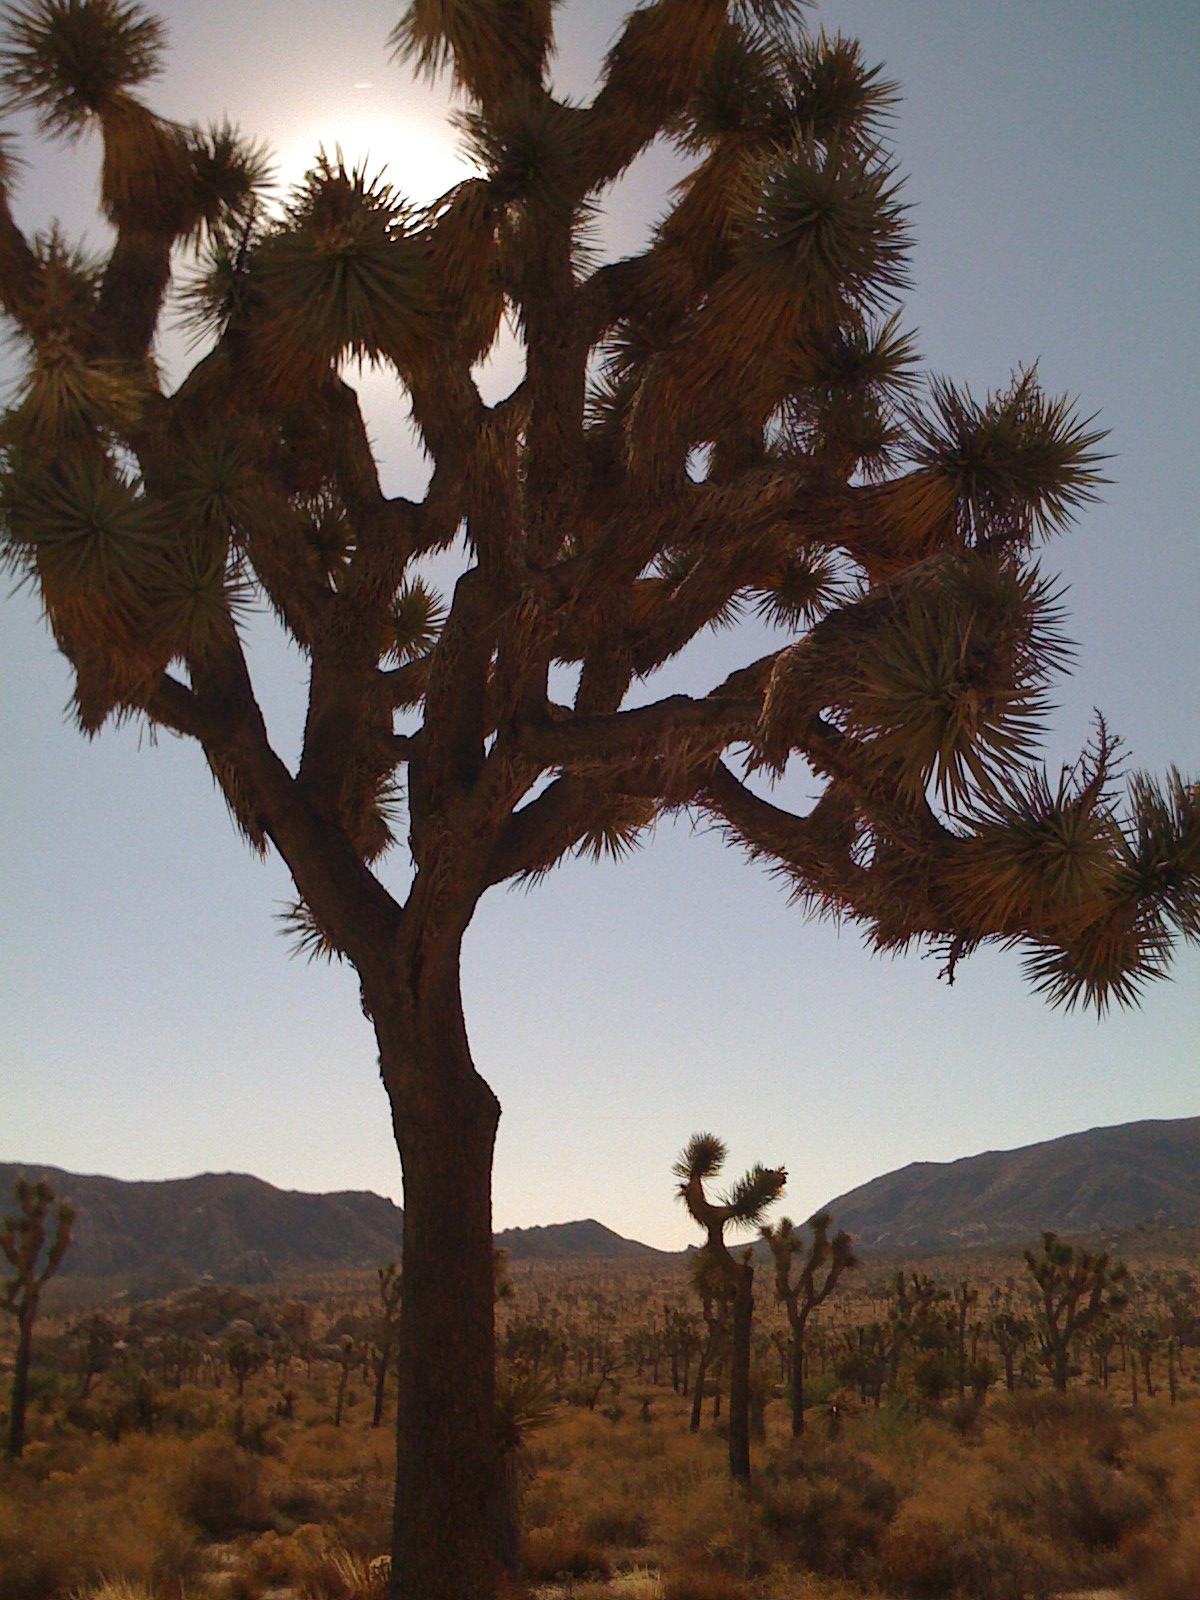
\includegraphics[width=.5\linewidth]{gfx/sagmeisterJoshuaTrees}}
	\end{center}
		\caption[Joshua Trees \newline \citep{Sagmeister:2008}]{Joshua Trees, die einzigen Schattenspender in der Mojave Wüste, gelten als Leitbilder für das Joshua Tree Principle, welches die Wirkungsweise von Guiding Principles beschreibt.}\label{fig:sagmeisterJoshuaTrees}
\end{figure}

Um die Wirkungsweise von Guiding Principles (im Sinne von Memen) zu veranschaulichen, soll eine kurze Geschichte helfen. 

\begin{quote}
	\textsl{>>Vor nicht all zu langer Zeit reiste ich durch die Wüstenlandschaften von Kalifornien, Arizona, Nevada und Utah. Dabei passierte ich einen Teil der Mojave Wüste, welche die 4 Bundesstaaten verbindet. Die Besonderheit dieser Wüstenlandschaft sind die dort wachsenden Joshua Trees\index{Joshua Trees} [vgl. \autoref{fig:sagmeisterJoshuaTrees}]. Sie waren seit jeher für die Einheimischen sehr wertvoll, da sie in der endlos scheinenden Wüstenlandschaft Schatten spendeten, wie mir der Tourguide erklärte. Bevor jedoch die Reiseleitung überhaupt begonnen hatte über die Joshua Trees zu sprechen, wusste ich bereits über sie Bescheid und erkannte sie. Nicht weil ich in meiner Freizeit Naturbücher auswendig lerne, sondern weil ich ironischer weise kurz vor meinem Reiseantritt ein Buch über Design von der Autorin Robin Williams gelesen habe. Sie beschreibt in ihrem Buch ein Prinzip auf welches ich mit meiner Geschichte ebenfalls hinzielen möchte: The Joshua Tree Principle. Wäre ich vor meiner Reise bereits in dieser Region unterwegs gewesen, wären mir die Bäume mit großer Sicherheit nie aufgefallen. Doch kaum wusste ich den Namen, wurde mir der Baum bewusst.<<}
\begin{flushright}\citep{Sagmeister:2008}\end{flushright}
\end{quote}

Genau das ist auch der Punkt:

\begin{quote}
	\textsl{>>Once you can name something, you’re conscious of it. You have power over it. You own it. You’re in control.<<}
\begin{flushright}\citep{Williams:1994}\end{flushright}
\end{quote}

Dawkin möchte ebenfalls mit dem Begriff Memen auf dieses Phänomen hinzielen: 

\begin{quote}
	\textsl{>>A meme should be regarded as a unit of information residing in a brain.<<}
	\begin{flushright}\citep{Dawkins:1982}\end{flushright}
	\smallskip
	\textsl{>>Meme can propagate themselves from brain to brain, from brain to book, from book to brain, from brain to computer, from computer to computer.<<}
	\begin{flushright}\citep{Dawkins:1986}\end{flushright}
\end{quote}

Durch das Wissen um Guiding Principles und die Fähigkeit sie benennen zu können, sollte es uns also möglich sein, sie kontrolliert einzusetzen, um das richtige Design zu kreieren. Wie kommt es dann aber, dass schlechtes Design keine Seltenheit ist? Guiding Principles sind Meme, die Designer in ihr Konsortium, welches aus vielen Memen besteht, aufnehmen. Abgesehen davon, dass Guiding Principles nur in bestimmten Kontexten wirken, können Entwickler Meme besitzen, die sie daran hindern ein gutes Design zu erstellen. Das können z.B. Meme über die Unternehmensorganisation, die Arbeit an sich oder das Umfeld sein. Das >>Sammeln<< von Memen, die zu einem guten Design führen, ist ein Lernprozess und unterscheidet somit ausgebildete Designer von Nicht- Designern. \\
Da nun klar ist, was Guiding Principles sind und wie sie wirken, wird in weiterer Folge auf einige Prinzipien des Interface Designs eingegangen. Über die Jahre wurden viele Design Prinzipien oder auch sog. Goldene Regeln des Designs entwickelt. Ihr Ursprung liegt dabei in der Psychologie und im Sammeln praktischer Erfahrungen. Ein Vorreiter auf diesem Gebiet war der Kognitionswissenschafter und Informatikprofessor Don Norman, der bereits 1988 mit seinem Bestseller The Design of Everyday Things \citep{Norman:1988} auf die Schwächen und Stärken von Designs hindeutete. Viele Designer und Autoren wie Williams, Shneiderman, oder Benyon bauten auf diese auf und erstellten darauf hin ihre eigenen aus Erfahrungen zusammengetragenen Prinzipien - einige vage, einige detaillierter formuliert. Angewendet, sollen sie im Allgemeinen helfen ein System zu lernen, das Gefühl geben stets die Kontrolle zu haben und vor Unsicherheit vorbeugen.

\begin{small}
\begin{enumerate}
	\item \emph{Bewahre die Konsistenz}\index{Guiding Principles!Konsistenz} - Diese Regel ist die meist missachtete. Unter anderem vielleicht weil es viele verschiedene Formen der Konsistenz gibt. Konsistenz sollte bei Standardoperationen und Repräsentationen, sowie bei der Benützung von Metaphern eingesetzt werden – innerhalb Applikationen und zwischen Applikationen. Sie hilft den	Benutzer ein mentales Modell eines Systems zu erstellen und es zu erhalten.\\
Ähnliche Situationen erfordern konsistente Aktionsabläufe; Bezeichnungen sollten in	Eingabeaufforderungen, Menüs und in der Hilfefunktion ident sein; Auf gleiche Farben, Layouts, Großschreibungen, Schriftarten usw. sollte durchgehend geachtet werden. Ausnahmen, wie das >>Nichtzeigen<< von Passwörtern oder das Bestätigen von Löschaktionen, sollten in ihrer Anzahl minimal gehalten werden.
	\item \emph{Gib Feedback}\index{Guiding Principles!Feedback} - Biete dem Benutzer für jede Aktion (so schnell wie möglich) genügend informatives Feedback, um ihm zu zeigen welchen Effekt seine Aktion hat. Für kleine, häufige Aktionen kann die Rückmeldung bescheiden ausfallen, wobei bei seltenen Haupttätigkeiten ein umfangreicheres Feedback gegeben werden sollte.
	\item \emph{Entwickle für Fehlverhalten}\index{Guiding Principles!Fehlverhalten} - Eine übliche Ausrede für auftretende Systemprobleme, ist das menschliche Fehlverhalten. Da irren jedoch menschlich ist, und Menschen Fehler machen müssen um zu lernen, sollte ein System so gut wie möglich designed werden, um	ernste Fehler zu vermeiden bzw. das Auftreten von Fehler so gering wie möglich zu halten. Beispiele wären Auswahlmenüs um Formulare auszufüllen oder das Ignorieren von	Buchstaben in numerischen Eingabefeldern. Falls Fehler trotzdem gemacht werden,	sollten simple, konstruktive Anweisungen geboten werden um das Problem zu lösen. Man	spricht hierbei auch von >>guten Fehlermeldungen<<.
	\item \emph{Zeig Toleranz}\index{Guiding Principles!Toleranz} - Gestatte Benutzern ihre Aktionen, insbesondere Fehler rückgängig zu machen. Diese Funktion nimmt die Angst von den Usern und ermutigt sie zur Erforschung von neuen Optionen.
	\item \emph{Übergib die Kontrolle}\index{Guiding Principles!Kontrolle} - Benutzer haben das Verlangen stets die Kontrolle über das	System zu haben. Unerwartete Systemaktionen führen zu Angst und Unbehagen. Deswegen sollte immer klar gemacht werden wer oder was gerade die Kontrolle besitzt,	um an das Vertrauen des Benutzers zu gelangen.
	\item \emph{Vereinfache die Programmstruktur}\index{Guiding Principles!Programmstruktur} - Laut dem Psychologen George Miller können sich	Menschen maximal 7±2 verschiedene Informationen merken (laut mancher Literatur sogar weniger). Er spricht dabei auch von der magischen Zahl 7\index{Die magische Zahl 7}. Aus diesem Grund sollte die Beanspruchung des Kurzzeitgedächtnisses minimal gehalten werden. Viele Entwickler halten sich strikt an diese Zahl z.B. beim Anzeigen von Items, vergessen jedoch, dass die Information meistens sowieso am Bildschirm zu sehen ist. Auf die Informationen kann also stets zurückgegriffen werden, ohne sie sich merken zu müssen. Es ist also nicht nötig Millers Theorie wörtlich im Design zu übernehmen, jedoch sollte eine Anwendung immer nur so komplex wie nötig und nicht wie möglich sein. Ein Beispiel wäre das Versenden einer Email. Die benötigte Information hierbei ist die Absender- und Empfängeradresse. Es wäre jedoch unnötig die Absenderadresse jedes Mal erneut einzugeben - Der Email-Client kümmert sich darum. Die Komplexität wurde somit aus der Sicht des Benutzers verringert.
	\item \emph{Vermittle Vertrautheit}\index{Guiding Principles!Vertrautheit} - Sprache und Symbole sollten immer so gewählt werden, damit sie für den Benutzer vertraut wirken. An Stellen wo dies nicht möglich ist, weil die	Konzepte so sehr von dem abweichen was die Benutzer kennen, sollten Metaphern verwendet werden (Beispiel: Papierkorb am Desktop). Sie stellen eine Verbindung zu bestehenden Wissen, einer vertrauten Quelle her. Im Allgemeinen sollten Elemente so	designed werden, dass immer Klarheit herrscht wofür sie stehen. Buttons müssen z.B.	aussehen wie Buttons, damit Benutzer wissen, dass man sie drücken muss.
	\item \emph{Achte auf Sichtbarkeit}\index{Guiding Principles!Sichtbarkeit} – Es sollte stets sichergestellt werden, dass Elemente sichtbar sind, damit der Benutzer sehen kann welche Funktionen verfügbar sind und mit welcher Aufgabe das System gerade beschäftigt ist. Dies basiert auf der psychologischen Grundregel, dass es einfacher ist etwas zu erkennen als sich daran erinnern zu müssen.
	\item \emph{Erstelle Grenzen}\index{Guiding Principles!Grenzen} - Grenzen sollen Benutzern das Gefühl geben, dass es nur einen möglichen Weg gibt - den richtigen natürlich. Sie bewahren User davor, unangebracht zu handeln indem sie ernste Fehler durch >>normale<< Tätigkeiten hervorrufen.\\
	Und schlussendlich..
	\item \emph{Sei freundlich}\index{Guiding Principles!Freundlichkeit} – Interaktive Systeme sollten höflich, freundlich, und angenehm gestaltet sein. Nichts ruiniert die Erfahrung mit einer Anwendung mehr als eine aggressive Mitteilung oder abrupte Unterbrechungen.
\end{enumerate}
\end{small}
\citep{Benyon:2005, Preece:1994, Saffer:2007, Shneiderman:1998}

\section*{Zusammenfassung}
Design ist ein alltäglicher und weitgehender Begriff, der sowohl Bedeutung als Tätigkeit und als Repräsentation in sich trägt. Es gibt viele verschiedene Designdisziplinen welche zur Unterscheidung von Kompetenzen professioneller Designer dienen. Ein wichtiger Bereich für Softwaredesign ist (User) Interface Design bzw. Interaction Design, welche sich besonders mit den subjektiven und qualitativen Aspekten, bei der Interaktion von Menschen und Computer, beschäftigen. Es gibt verschiedenste Methoden, die benutzt werden können um Designprobleme zu verstehen und um nötige Lösungsstrategien zu entwickeln. Skizzen bieten durch ihre minimale Detailstufe und der kurzen Herstellungszeit Mehrdeutigkeiten, die zum Weiterforschen und Kommentieren anregen. Dieser soziale Prozess ist wichtig in der Ideenfindung am Anfang einer Designphase. Prototypen verbinden alle Teile eines Designs, zu einer Einheit und verschaffen im (User) Testing neue Einblicke. Beobachtungen von Verhaltensmustern innerhalb der Testings bewegen schlussendlich dazu das Design iterativ zu überarbeiten. Es kann zusätzlich auch nützlich sein, sich durch Personas und Szenarien eine Art Leitfaden zusammen zu stellen, der durch das Beleuchten von Tätigkeiten potentieller Benutzer zustande kommt. Dieser sollte aber ständig vervollständigt werden, da er meist Lücken aufweist. Es gibt kein Rezept für das \emph{richtige} Design, jedoch entstanden über die Jahre sog. Guiding Prinicples oder Leitfäden, die Designern helfen sollen bessere Systeme zu entwickeln. \\
Design hängt immer mit der Kommunikation und Interaktion von Personen zusammen und ist somit eine >>soziale Konstruktion einer technischen Realität<<. Das folgende Kapitel soll nun näher auf den kollaborativen Charakter eingehen.

